\documentclass[11pt,a4paper]{article}

\usepackage[T1]{fontenc}
\usepackage[margin=2.4cm]{geometry}
\usepackage{times}
\usepackage{graphicx}
\usepackage{booktabs}
\usepackage{array}
\usepackage{amsmath}
\usepackage{amssymb}
\usepackage[hyphens]{url}
\usepackage{hyperref}
\usepackage{setspace}
\usepackage{caption}
\usepackage{float}
\usepackage{enumitem}

\hypersetup{colorlinks=true,linkcolor=black,citecolor=black,urlcolor=blue}
\captionsetup{font=small,labelfont=bf,skip=6pt}
\setstretch{1.18}
\graphicspath{{../results/plots/}}
\setlength{\parskip}{0.45em}
\setlength{\parindent}{1.2em}

\title{\vspace{-1.2em}Evaluating NLI Models under Disagreement:\\
DeBERTa-v3 and ModernBERT on ChaosNLI\vspace{-0.4em}}
\author{Dujana Abrar \and Jiayin Feng}
\date{}

\begin{document}
\maketitle
\vspace{-1.2em}

\begin{abstract}
Natural language inference (NLI) benchmarks usually keep one gold label per example, even though people often disagree. ChaosNLI (Collective Human Opinions in oft-used NLI evaluation sets) collected 100 labels for 1,514 SNLI and 1,599 MNLI-matched items and scores models against that human distribution as well as against the majority vote. Prior work showed that BERT, RoBERTa, XLNet, BART, and ALBERT match those distributions poorly, and that accuracy drops close to chance once annotators split. This report tests two later public NLI checkpoints, DeBERTa-v3 and ModernBERT, with the same metrics. We find that the two models do not move in the same direction. DeBERTa-v3 reaches the highest majority-label accuracy on ChaosNLI-SNLI (79.3\%, versus 78.7\% for RoBERTa-large) but has the worst Jensen--Shannon distance (JSD) and Kullback--Leibler (KL) divergence of any model we compare. ModernBERT has the lowest JSD and KL divergence, including on MNLI, while remaining below RoBERTa on majority accuracy. Both models stay overconfident on high-disagreement items, and they often pick the same label there. Softening the softmax with temperature scaling cuts JSD without changing any predicted label, so a large part of the distribution error is sharpness rather than a wrong ranking. Majority accuracy and distribution matching remain different skills. Extra NLI training data does not, on its own, improve the second.
\end{abstract}

\section{Introduction}

Natural language inference (NLI) asks whether a hypothesis is entailed by a premise, contradicts it, or is neither. SNLI \cite{bowman2015snli} and MNLI \cite{williams2018mnli} treat each pair as having one correct label, usually the majority of a handful of annotators. That setup hides a lot of real disagreement. ChaosNLI \cite{nie2020chaosnli} re-annotated 1,514 SNLI and 1,599 MNLI-matched development examples with 100 labels each. A fair number of original majority labels do not match the 100-annotator majority, and many items have high label entropy.

Nie et al.\ \cite{nie2020chaosnli} compared BERT, RoBERTa, XLNet, BART, and ALBERT against those 100-way distributions. Two results from that paper still matter here. Models that did well on ordinary accuracy were not the ones that matched the human distribution, measured by Jensen--Shannon distance (JSD) and Kullback--Leibler (KL) divergence. Accuracy was high when annotators already agreed and close to chance when they did not. Most remaining errors sat in the low-agreement slice. If later NLI models keep improving majority accuracy, it is not obvious that they also get better at representing disagreement.

We evaluate two encoder checkpoints released after the ChaosNLI study by Nie et al., DeBERTa-v3 and ModernBERT, and compare them with the encoder baselines reported in that work. Both checkpoints were fine-tuned on multiple NLI datasets. This makes them useful for examining whether newer NLI checkpoints differ in how well they match human label distributions. Neither model was trained directly to predict the 100-annotator distributions used by ChaosNLI. Their architectures and training mixes differ, so they may also differ in how they represent uncertainty, even when majority-label accuracy looks similar.

We keep the original ChaosNLI metrics: JSD, KL divergence, old accuracy (original dataset label), and new accuracy (100-annotator majority). These metrics allow us to compare the models with the results reported in the original ChaosNLI study. We also split examples by annotation entropy, compare the two checkpoints with each other, and apply temperature scaling when model confidence and human uncertainty come apart.

This is an error and generalization analysis of existing models, not a new training method. We run two frozen public checkpoints on ChaosNLI-SNLI and ChaosNLI-MNLI-matched and look at where they are strong, where they fail, and whether SNLI-style performance carries over to MNLI.

The rest of the report is organized around three questions:
\begin{itemize}[itemsep=0.4em, topsep=0.4em]
    \item How well do these two checkpoints match ChaosNLI human label distributions, relative to the 2020 encoder baselines?
    \item Does higher majority-label accuracy also mean a better match to human disagreement?
    \item Does model confidence track human uncertainty, and can a simple post-hoc calibration step improve the distribution scores without changing predicted labels?
\end{itemize}

\section{Related Work}

Research on disagreement in NLI has moved from questioning the use of a single gold label toward evaluating and modeling distributions of human judgments. The following sections review this development, from human disagreement and ChaosNLI to approaches for modeling and calibrating human opinion distributions, and finally to recent NLI models and the remaining gap.

\subsection{Human disagreement in NLI and ChaosNLI}

Human disagreement has been studied in NLI because of the difficulty of assigning a single label to some sentence pairs. Pavlick and Kwiatkowski \cite{pavlick2019inherent} showed that disagreements between annotators often persist even when more judgments are collected and argued that they cannot simply be treated as annotation noise. They also found that the uncertainty expressed by NLI models does not necessarily correspond to human uncertainty. Their work highlights the need to consider more than a single aggregate label when evaluating NLI models.

ChaosNLI \cite{nie2020chaosnli} builds on this idea by collecting 100 annotations for selected examples from SNLI, MNLI-matched, and $\alpha$NLI. The resulting label distributions make it possible to assess how closely model predictions reflect the range of human judgments. The ChaosNLI majority label differs from the original dataset label for 24.97\% of SNLI examples and 31.77\% of MNLI-matched examples. The level of human disagreement also varies considerably across examples.

Nie et al.\ \cite{nie2020chaosnli} compared several NLI models, including BERT, RoBERTa, XLNet, BART, ALBERT, and DistilBERT, using both accuracy and distributional measures such as JSD and KL divergence. DistilBERT achieved comparatively strong KL scores and weak accuracy. The authors interpreted this as evidence that majority classification and distribution matching are not the same skill. They also found that model accuracy decreased as human disagreement increased. These results show why both distributional matching and majority-label accuracy are relevant when evaluating models under human disagreement.

\subsection{Modeling and calibrating human disagreement}

Later work explored ways to make NLI models better represent human disagreement. Zhou et al.\ \cite{zhou2022distributed} introduced Distributed NLI, where models predict the distribution of human judgments instead of a single label. They showed that methods such as recalibration and distribution estimation can improve the match between model predictions and human opinion distributions. However, the best results remained below the estimated human upper bound.

Meissner et al.\ \cite{meissner2021capturing} changed the training target from a single gold label to a human label distribution. Their results indicated that training on these distributions can reduce JSD on ChaosNLI. Wang et al.\ \cite{wang2022calibrated} took a different approach and focused on calibration. They found that label smoothing and temperature scaling can help model probabilities capture the distribution of human judgments.

Baan et al.\ \cite{baan2022stop} studied calibration when human annotators disagree. They argued that ordinary calibration metrics based on a single majority label are misleading when the ground truth itself is a distribution. They proposed measures that take the full human judgment distribution into account.

Lee et al.\ \cite{lee2023dissenting} evaluated instruction-tuned language models on ChaosNLI and found that these models struggled to match human disagreement distributions. For example, GPT-3 did not beat RoBERTa-large on JSD. Their study focuses on generative models and does not evaluate the two encoder checkpoints we use.

Overall, these studies show that majority-label prediction and human-distribution matching are different goals. They also suggest that calibrating model probabilities can improve distributional matching.

\subsection{Recent NLI models and the remaining gap}

Since the original ChaosNLI study, newer NLI checkpoints have been developed and some have also been evaluated under human disagreement. Tao et al.\ \cite{tao2026confidence}, for example, evaluated DeBERTa-v3-base and RoBERTa-large on ChaosNLI and compared several post-hoc calibration methods. Their study provides a recent reference for evaluating model confidence when human annotators disagree. However, the DeBERTa-v3-base checkpoint differs from the large multi-dataset DeBERTa-v3 checkpoint used in our experiments, and their study does not include ModernBERT.

The two newer NLI checkpoints evaluated in our study are:

\begin{itemize}[itemsep=0.4em, topsep=0.4em]
\item \textbf{DeBERTa-v3} \cite{he2023debertav3,laurer2024less}. Fine-tuned on MNLI, FEVER-NLI, ANLI, LingNLI, and WANLI. SNLI was left out of training because of known label issues. Checkpoint: \path{MoritzLaurer/DeBERTa-v3-large-mnli-fever-anli-ling-wanli}.
\item \textbf{ModernBERT} \cite{warner2024modernbert,sileo2024tasksource}. Multi-task fine-tuned on a large set of NLI-format datasets, including MNLI, ANLI, WANLI, LingNLI, SICK, and several logic and document NLI tasks. Checkpoint: \path{tasksource/ModernBERT-large-nli}.
\end{itemize}

The two checkpoints differ in both architecture and the NLI datasets used for fine-tuning. Both include WANLI (Worker-AI Collaboration for NLI), which was created through human-AI collaboration to construct challenging NLI examples \cite{liu2022wanli}. Importantly, neither checkpoint was trained to predict the 100-annotator label distributions used by ChaosNLI.

To our knowledge, neither of these checkpoints has been evaluated on ChaosNLI using the original distributional metrics. We also found no ChaosNLI results for either checkpoint in their Hugging Face model cards. Our study extends this line of work by evaluating DeBERTa-v3 and ModernBERT against the full human label distributions in ChaosNLI.

\section{Dataset}

We use two subsets of ChaosNLI \cite{nie2020chaosnli}: ChaosNLI-SNLI and ChaosNLI-MNLI-matched. ChaosNLI-SNLI contains 1,514 examples and ChaosNLI-MNLI-matched contains 1,599. Each example has 100 crowd labels, a majority label, a normalized label distribution over entailment, neutral, and contradiction, and the original SNLI or MNLI label. We do not use ChaosNLI-$\alpha$NLI. The selected checkpoints are 3-way NLI classifiers, not abductive two-choice models.

Human entropy is computed from the 100-label distribution, in bits. Mean entropy is 0.80 on SNLI and 1.07 on MNLI. A quarter of SNLI items have entropy above 1 bit; on MNLI that share is 64\%. The original dataset label disagrees with the 100-annotator majority on 25\% of SNLI items and 32\% of MNLI items. ChaosNLI-SNLI majority labels are skewed toward neutral (813 N, 421 E, 280 C). ChaosNLI-MNLI majority labels are skewed toward entailment (741 E, 583 N, 275 C). That shift matters later: both modern models lose a lot of entailment recall when they move from SNLI to MNLI.

We split each subset into tertiles of human entropy and call them low, medium, and high disagreement. On SNLI the cuts fall at 0.68 and 0.97 bits; on MNLI they fall at 0.99 and 1.19 bits. The high-entropy SNLI bin is therefore an easier cut than the high-entropy MNLI bin. The 2020 baseline predictions come from the official ChaosNLI release. We recompute JSD, KL, and both accuracies from those files so that our numbers sit on the same protocol as the published scoreboard.

\section{Methods}

We evaluate DeBERTa-v3 and ModernBERT on ChaosNLI using classification, distributional measures, and qualitative analysis. Their predictions are compared with the human label distributions and the original ChaosNLI baselines. We also analyze model confidence and agreement between the two checkpoints. Finally, temperature scaling is used to test whether adjusting model confidence improves distributional matching without changing the predicted labels.

\subsection{Model inference}

We load both models with Hugging Face Transformers and run them in evaluation mode. No weights are updated on ChaosNLI. Premises and hypotheses are tokenized as pairs, with padding and truncation. We do not set a custom maximum length, so each model uses its own tokenizer default (512 for DeBERTa-v3, 8192 for ModernBERT).

For each example, we obtain a probability distribution over the three NLI classes using softmax. The probabilities are aligned to the order (entailment, neutral, contradiction). The predicted label is the class with the highest probability:
\[
\hat{y} = \arg\max_i p_i.
\]
Confidence is defined as the maximum class probability:
\[
c = \max_i p_i.
\]

We keep the full probability distribution because it is required for the distributional metrics and uncertainty analysis. For each example, we store the predicted label, probability distribution, and confidence. Default batch size is 32. We do not use dropout at test time, and we do not ensemble.

\subsection{Evaluation metrics}

We first evaluate whether the model prediction matches the reference label using two accuracy measures. Old accuracy compares the model to the original dataset label. New accuracy compares it to the ChaosNLI majority.

Accuracy only considers the predicted label and does not capture the full distribution of human judgments. We therefore use KL divergence and JSD to compare the model probability distribution with the human label distribution.

KL divergence measures the difference between two probability distributions. In our evaluation, it is computed as
\[
\mathrm{KL}(p_{\mathrm{human}} \Vert p_{\mathrm{model}})
\]
in nats. The human distribution is treated as the reference and the model distribution is evaluated against it. Smaller KL values indicate greater similarity between the two distributions.

JSD provides a symmetric comparison of the human and model distributions. We first compute their average distribution, then the Jensen--Shannon divergence (JSDiv). We then use SciPy's Jensen--Shannon distance, which is the square root of JSDiv and uses the natural log. This matches the ChaosNLI evaluation code:
\[
m=\frac{1}{2}\left(p_{\mathrm{human}}+p_{\mathrm{model}}\right),
\]
\[
\mathrm{JSDiv}(p_{\mathrm{human}}, p_{\mathrm{model}}) =
\frac{1}{2}\mathrm{KL}(p_{\mathrm{human}}\Vert m)
+
\frac{1}{2}\mathrm{KL}(p_{\mathrm{model}}\Vert m),
\]
\[
\mathrm{JSD}(p_{\mathrm{human}}, p_{\mathrm{model}})=\sqrt{\mathrm{JSDiv}(p_{\mathrm{human}}, p_{\mathrm{model}})}.
\]
Lower JSD values mean that the model is closer to the human distribution.

We further analyze model uncertainty using confidence and entropy. Model confidence is the maximum predicted class probability and captures how strongly the model favors its predicted label. Model entropy measures how the probability is distributed across the three NLI classes. It is computed in bits as
\[
H(p)=-\sum_i p_i\log_2 p_i.
\]
Higher entropy represents a more evenly spread prediction and greater model uncertainty. We calculate the mean confidence and mean model entropy across the examples.

In addition, we compute the Spearman correlation between model confidence and human entropy, and between model entropy and human entropy. These correlations examine whether model confidence or uncertainty changes in the same direction as human disagreement.

\subsection{Baselines and model--model comparison}

To compare our results with the original ChaosNLI evaluation, we use the prediction files provided for BERT-large, RoBERTa-large, XLNet-large, BART-large, and ALBERT-xxlarge. Their logits are converted to probability distributions with softmax. We recompute the JSD, KL divergence, old accuracy, and new accuracy from these predictions. Recomputed SNLI and MNLI scores match the published table to four decimals.

For each example, we record whether DeBERTa-v3 and ModernBERT predict the same label, and whether that shared label matches the human majority. We perform this comparison separately for the low-, medium-, and high-disagreement groups defined by human entropy. We then compare model consistency across these groups and check whether they make the same errors on ambiguous examples.

This comparison is not in the original ChaosNLI paper. The point is to see whether two independently trained modern NLI models fall back on the same convention when humans do not agree.

\subsection{Temperature scaling}

The saved prediction files store softmax probabilities, not raw logits, so we recover logits as $\log p$ before searching for a temperature $T$. We draw a random 50/50 split (seed 0), search $T \in [0.5, 5.0]$ in 19 equal steps to minimize JSD on one half, and score the other half. Argmax is invariant to $T>0$, so accuracy cannot change. We also search for a $T$ that matches mean model entropy to mean human entropy, without using labels.

\subsection{Qualitative analysis}

The selection of examples for the qualitative analysis is not random. We use targeted sampling based on specific properties of the model predictions and human disagreement. We compare the predictions of DeBERTa-v3 and ModernBERT and select examples that meet particular criteria.

Before describing these criteria, we clarify two terms. The SNLI and MNLI-matched datasets provide one label for each example. We refer to this as the \textit{original dataset label}. ChaosNLI provides a label distribution based on 100 annotations collected from crowd workers. The label with the highest proportion in this distribution is referred to as the \textit{human majority label}. The original dataset label and the human majority label do not always agree. This disagreement is used as a selection criterion in two cases described below.

High human entropy identifies examples with substantial annotator disagreement. These examples are useful for qualitative analysis, as they capture cases where human judgments diverge. High model confidence highlights cases where a model remains highly certain despite this disagreement. This allows us to inspect examples where the model distribution is much sharper than the human distribution.

Specifically, we use four selection criteria:

\begin{itemize}[itemsep=0.4em, topsep=0.4em]
\item high-entropy examples where DeBERTa-v3 and ModernBERT predict the same label with high confidence, but this label differs from the human majority label;
\item high-entropy examples where DeBERTa-v3 and ModernBERT predict different labels;
\item examples where the original dataset label differs from the human majority label, but both models predict the human majority label;
\item examples where the original dataset label differs from the human majority label, and both models predict the original dataset label.
\end{itemize}

For the first two criteria, we use a human entropy threshold of $1.0$. For the last two criteria, we use a threshold of $0.8$. The selected examples are manually inspected. Representative cases are then chosen to identify recurring patterns of model--human disagreement.

\section{Results}

We begin by comparing the two models with the original ChaosNLI baselines. We then look more closely at error tendencies, including confusion against the 100-annotator majority and cases where the original dataset label disagrees with that majority. The remaining analyses consider entropy bins, agreement between the two checkpoints, temperature scaling, and qualitative examples.

\subsection{Overall comparison}

Table~\ref{tab:snli} and Table~\ref{tab:mnli} report official ChaosNLI metrics. Lower JSD and KL are better. Higher accuracy is better.

\begin{table}[H]
\centering
\small
\caption{ChaosNLI-SNLI ($n=1514$). 2020 rows are recomputed from the official prediction files.}
\label{tab:snli}
\begin{tabular}{lcccc}
\toprule
Model & JSD $\downarrow$ & KL $\downarrow$ & Old acc.\ $\uparrow$ & New acc.\ $\uparrow$ \\
\midrule
BERT-large (2020) & 0.230 & 0.502 & 0.727 & 0.738 \\
RoBERTa-large (2020) & 0.221 & 0.494 & 0.749 & 0.787 \\
XLNet-large (2020) & 0.226 & 0.505 & 0.743 & 0.781 \\
BART-large (2020) & 0.220 & 0.471 & 0.742 & 0.783 \\
ALBERT-xxlarge (2020) & 0.235 & 0.534 & 0.715 & 0.781 \\
DeBERTa-v3 (ours) & 0.278 & 0.858 & 0.709 & 0.793 \\
ModernBERT (ours) & 0.214 & 0.378 & 0.708 & 0.768 \\
\bottomrule
\end{tabular}
\end{table}

\begin{table}[H]
\centering
\small
\caption{ChaosNLI-MNLI-matched ($n=1599$).}
\label{tab:mnli}
\begin{tabular}{lcccc}
\toprule
Model & JSD $\downarrow$ & KL $\downarrow$ & Old acc.\ $\uparrow$ & New acc.\ $\uparrow$ \\
\midrule
BERT-large (2020) & 0.315 & 0.845 & 0.612 & 0.569 \\
RoBERTa-large (2020) & 0.311 & 0.870 & 0.674 & 0.635 \\
XLNet-large (2020) & 0.312 & 0.882 & 0.674 & 0.619 \\
BART-large (2020) & 0.317 & 0.885 & 0.664 & 0.592 \\
ALBERT-xxlarge (2020) & 0.316 & 0.862 & 0.649 & 0.590 \\
DeBERTa-v3 (ours) & 0.364 & 1.465 & 0.695 & 0.634 \\
ModernBERT (ours) & 0.285 & 0.638 & 0.671 & 0.624 \\
\bottomrule
\end{tabular}
\end{table}

On SNLI, DeBERTa-v3 has the highest new accuracy (0.793) and the worst JSD and KL. Its old SNLI accuracy (0.709) is below RoBERTa-large (0.749). That split fits the model card: SNLI was not used in training. The checkpoint lines up better with the 100-annotator majority than with the original five-annotator labels, and still produces very peaked distributions (mean confidence 0.947, mean model entropy 0.21 bits, against human entropy 0.80).

ModernBERT has the best SNLI JSD (0.214) and KL (0.378), better than BART-large, which was the previous JSD leader in this set. Its new accuracy (0.768) is below RoBERTa-large.

On MNLI the 2020 models already sat near the chance JSD band (about 0.31). ModernBERT is the first model in Table~\ref{tab:mnli} to move clearly below that band (JSD 0.285, KL 0.638). DeBERTa-v3 improves old MNLI accuracy (0.695 vs.\ 0.674 for RoBERTa) and makes KL almost twice as large (1.465 vs.\ 0.870). New accuracy is essentially tied with RoBERTa (0.634 vs.\ 0.635).

Higher majority accuracy and better distribution match do not arrive together on these two checkpoints.

\subsection{Error tendencies}
\label{sec:errors}

Table~\ref{tab:conf-snli} and Table~\ref{tab:conf-mnli} are confusion matrices against the 100-annotator majority. Rows are the human majority. Columns are the model prediction.

\begin{table}[H]
\centering
\small
\caption{Confusion on ChaosNLI-SNLI against the 100-annotator majority.}
\label{tab:conf-snli}
\begin{tabular}{llccc}
\toprule
Model & Gold $\backslash$ Pred & E & N & C \\
\midrule
DeBERTa-v3 & E & 344 & 68 & 9 \\
 & N & 95 & 647 & 71 \\
 & C & 10 & 60 & 210 \\
\midrule
ModernBERT & E & 331 & 77 & 13 \\
 & N & 79 & 615 & 119 \\
 & C & 15 & 48 & 217 \\
\bottomrule
\end{tabular}
\end{table}

\begin{table}[H]
\centering
\small
\caption{Confusion on ChaosNLI-MNLI-matched against the 100-annotator majority.}
\label{tab:conf-mnli}
\begin{tabular}{llccc}
\toprule
Model & Gold $\backslash$ Pred & E & N & C \\
\midrule
DeBERTa-v3 & E & 382 & 340 & 19 \\
 & N & 45 & 410 & 128 \\
 & C & 6 & 48 & 221 \\
\midrule
ModernBERT & E & 383 & 330 & 28 \\
 & N & 42 & 399 & 142 \\
 & C & 17 & 43 & 215 \\
\bottomrule
\end{tabular}
\end{table}

On SNLI both models are strongest on entailment and neutral. DeBERTa-v3 recall is 0.82 / 0.80 / 0.75 for E / N / C. ModernBERT is 0.79 / 0.76 / 0.78. ModernBERT calls contradiction more often when the majority is neutral (119 vs.\ 71), which shows up as lower contradiction precision (0.62 vs.\ 0.72). That is a useful split: DeBERTa is the better SNLI majority classifier partly because it is more conservative about C.

MNLI looks different. Entailment recall falls to about 0.52 for both models. Contradiction recall stays high (0.80 DeBERTa, 0.78 ModernBERT). The missing entailment mass goes to neutral: DeBERTa predicts N on 340 of 741 majority-entailment items. Among DeBERTa errors, 388 of 586 are a predicted N. The same pattern holds for ModernBERT (373 of 602 errors). False-neutral rate on MNLI is 0.24 for DeBERTa and 0.23 for ModernBERT, against 0.08--0.09 on SNLI.

That is the main generalization result. SNLI is caption-style image descriptions. MNLI is multi-genre prose. Both checkpoints were trained on MNLI, so the drop is not from missing MNLI as a source. It lines up with the entropy gap (0.80 bits on SNLI vs.\ 1.07 on MNLI) and with the 32\% old-vs-new label mismatch on MNLI. The models keep a strong contradiction detector and become cautious on entailment, which is the opposite of the MNLI majority prior (entailment is the most common 100-annotator label).

When the original dataset label and the 100-annotator majority disagree, the two models do not follow the same source. On SNLI that happens for 378 items. DeBERTa-v3 matches the new majority on 65\% of them and the old label on 31\%. ModernBERT is 60\% new / 36\% old. On MNLI the mismatch set is 508 items, and both models flip: they follow the original MNLI label more often than the ChaosNLI majority (DeBERTa 58\% old / 39\% new; ModernBERT 56\% old / 41\% new). SNLI was left out of DeBERTa training because of label quality, and the checkpoint does prefer the re-annotation there. MNLI was in training for both models, and they stick closer to the older convention even when 100 annotators vote the other way.

\subsection{Entropy bins}

Table~\ref{tab:bins-acc} shows new accuracy by human-entropy tertile. Figure~\ref{fig:snli-acc} and Figure~\ref{fig:snli-jsd} plot the SNLI split. Figure~\ref{fig:mnli-acc} and Figure~\ref{fig:mnli-jsd} show the same split on MNLI.

\begin{table}[H]
\centering
\small
\caption{New accuracy by human-disagreement tertile.}
\label{tab:bins-acc}
\begin{tabular}{lccc}
\toprule
Split & Low & Medium & High \\
\midrule
SNLI DeBERTa-v3 & 0.948 & 0.820 & 0.612 \\
SNLI ModernBERT & 0.926 & 0.781 & 0.598 \\
SNLI RoBERTa-large & 0.952 & 0.806 & 0.602 \\
MNLI DeBERTa-v3 & 0.705 & 0.619 & 0.576 \\
MNLI ModernBERT & 0.711 & 0.584 & 0.576 \\
MNLI RoBERTa-large & 0.704 & 0.636 & 0.567 \\
\bottomrule
\end{tabular}
\end{table}

On high-disagreement items, all three models are around 60\% on SNLI and 57\% on MNLI. The low-entropy SNLI bin is nearly solved (about 95\%). That is the same shape Nie et al.\ reported. The newer encoders do not move the high-entropy slice.

Mean confidence on SNLI stays high for DeBERTa-v3 even when humans disagree (0.978 / 0.946 / 0.918 across the three bins). ModernBERT drops more (0.924 / 0.850 / 0.795), which is one reason its JSD is lower. On MNLI, Spearman $\rho$ between DeBERTa confidence and human entropy is $-0.05$. For ModernBERT it is $-0.17$. Neither softmax is a reliable signal of MNLI ambiguity.

\begin{figure}[H]
\centering
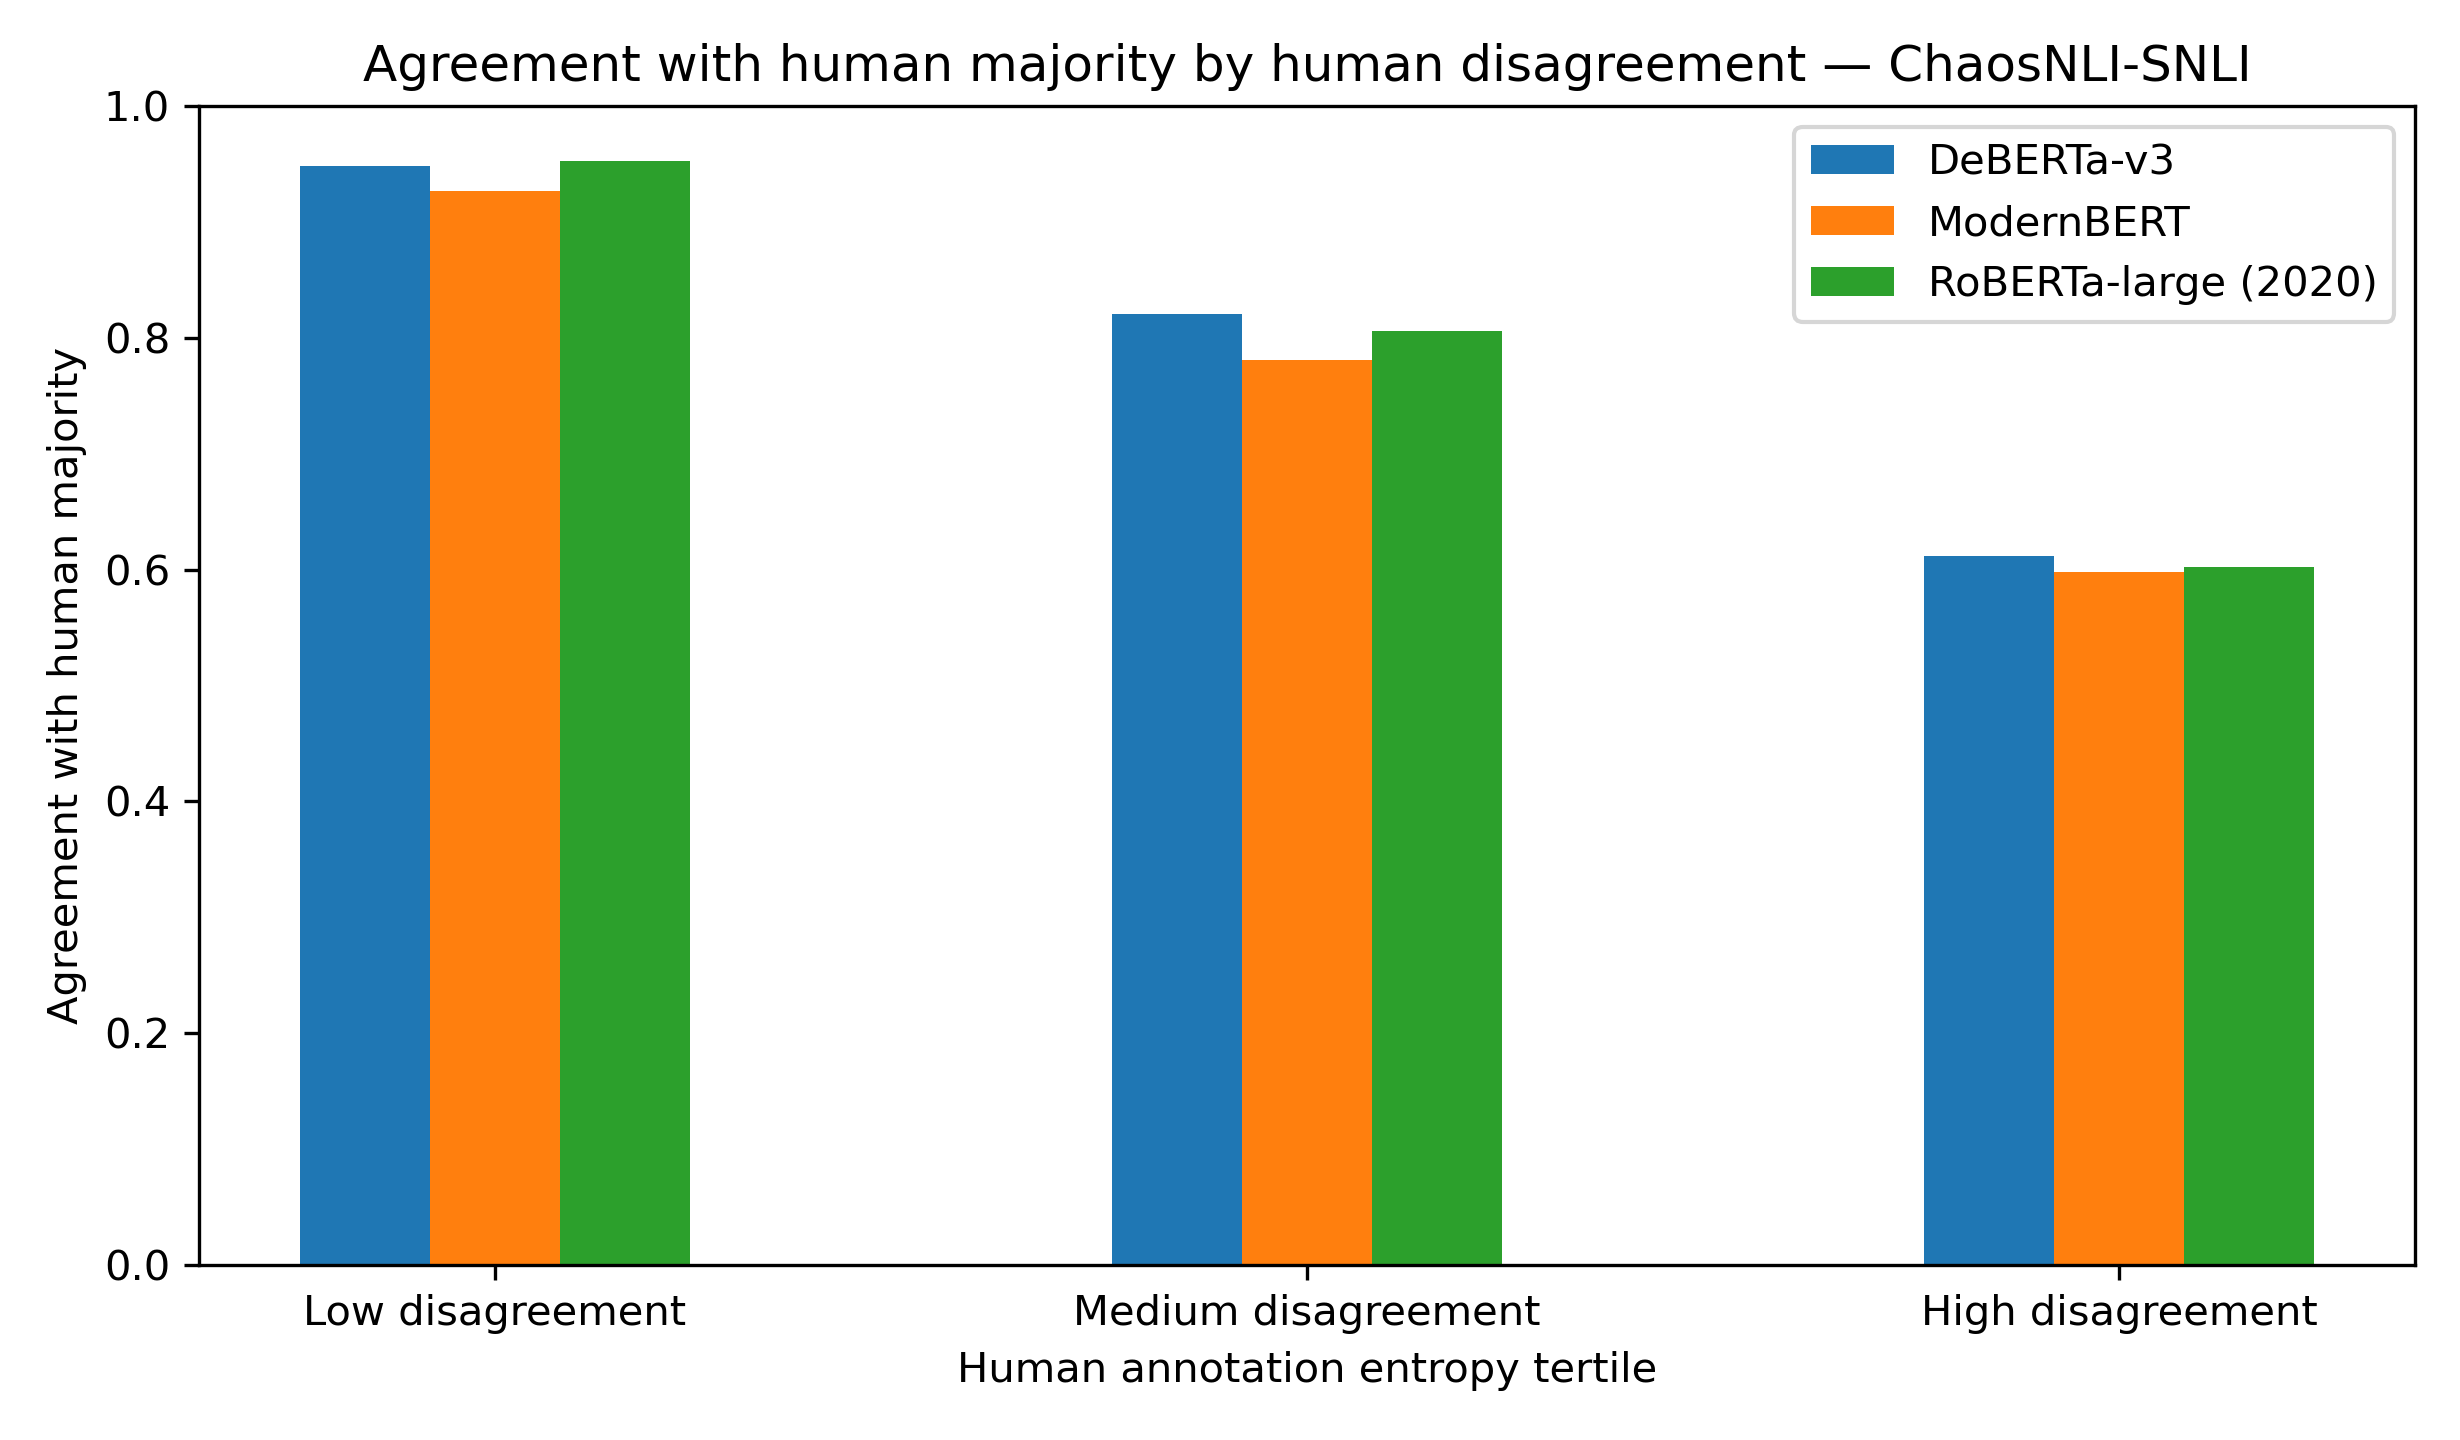
\includegraphics[width=0.85\textwidth]{snli_new_acc_by_entropy.png}
\caption{Agreement with the 100-annotator majority by human-disagreement tertile on ChaosNLI-SNLI.}
\label{fig:snli-acc}
\end{figure}

\begin{figure}[H]
\centering
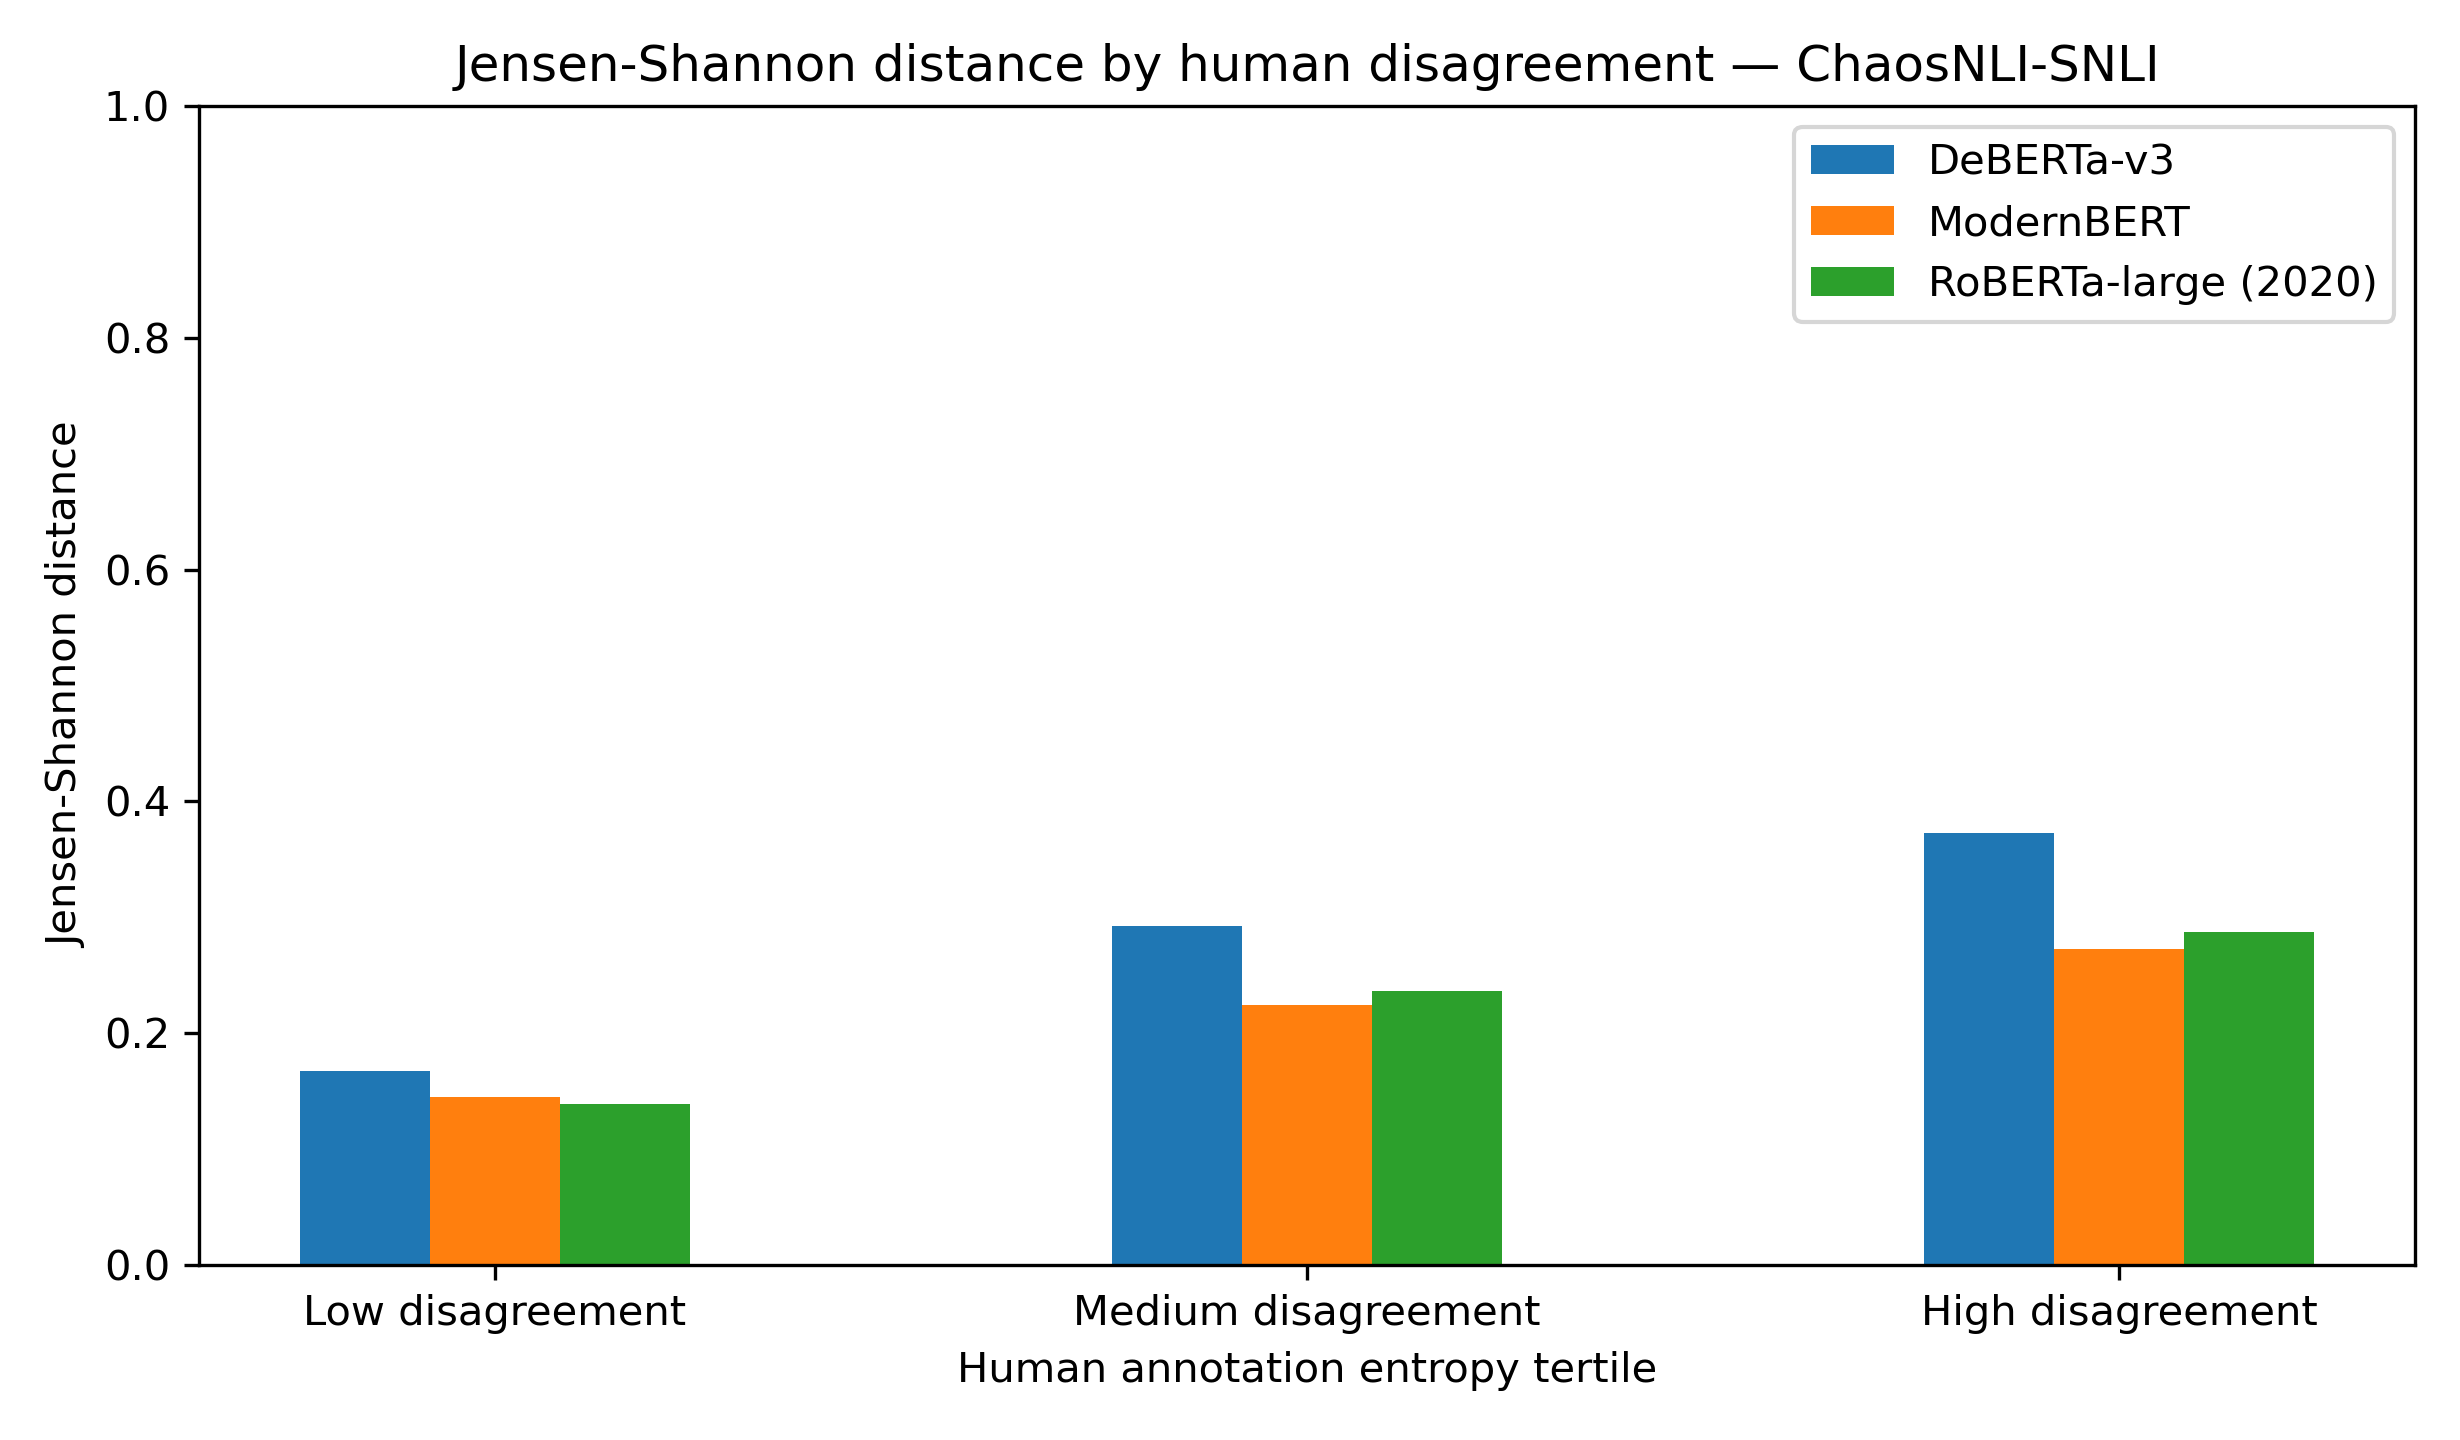
\includegraphics[width=0.85\textwidth]{snli_jsd_by_entropy.png}
\caption{Jensen--Shannon distance by human-disagreement tertile on ChaosNLI-SNLI.}
\label{fig:snli-jsd}
\end{figure}

\begin{figure}[H]
\centering
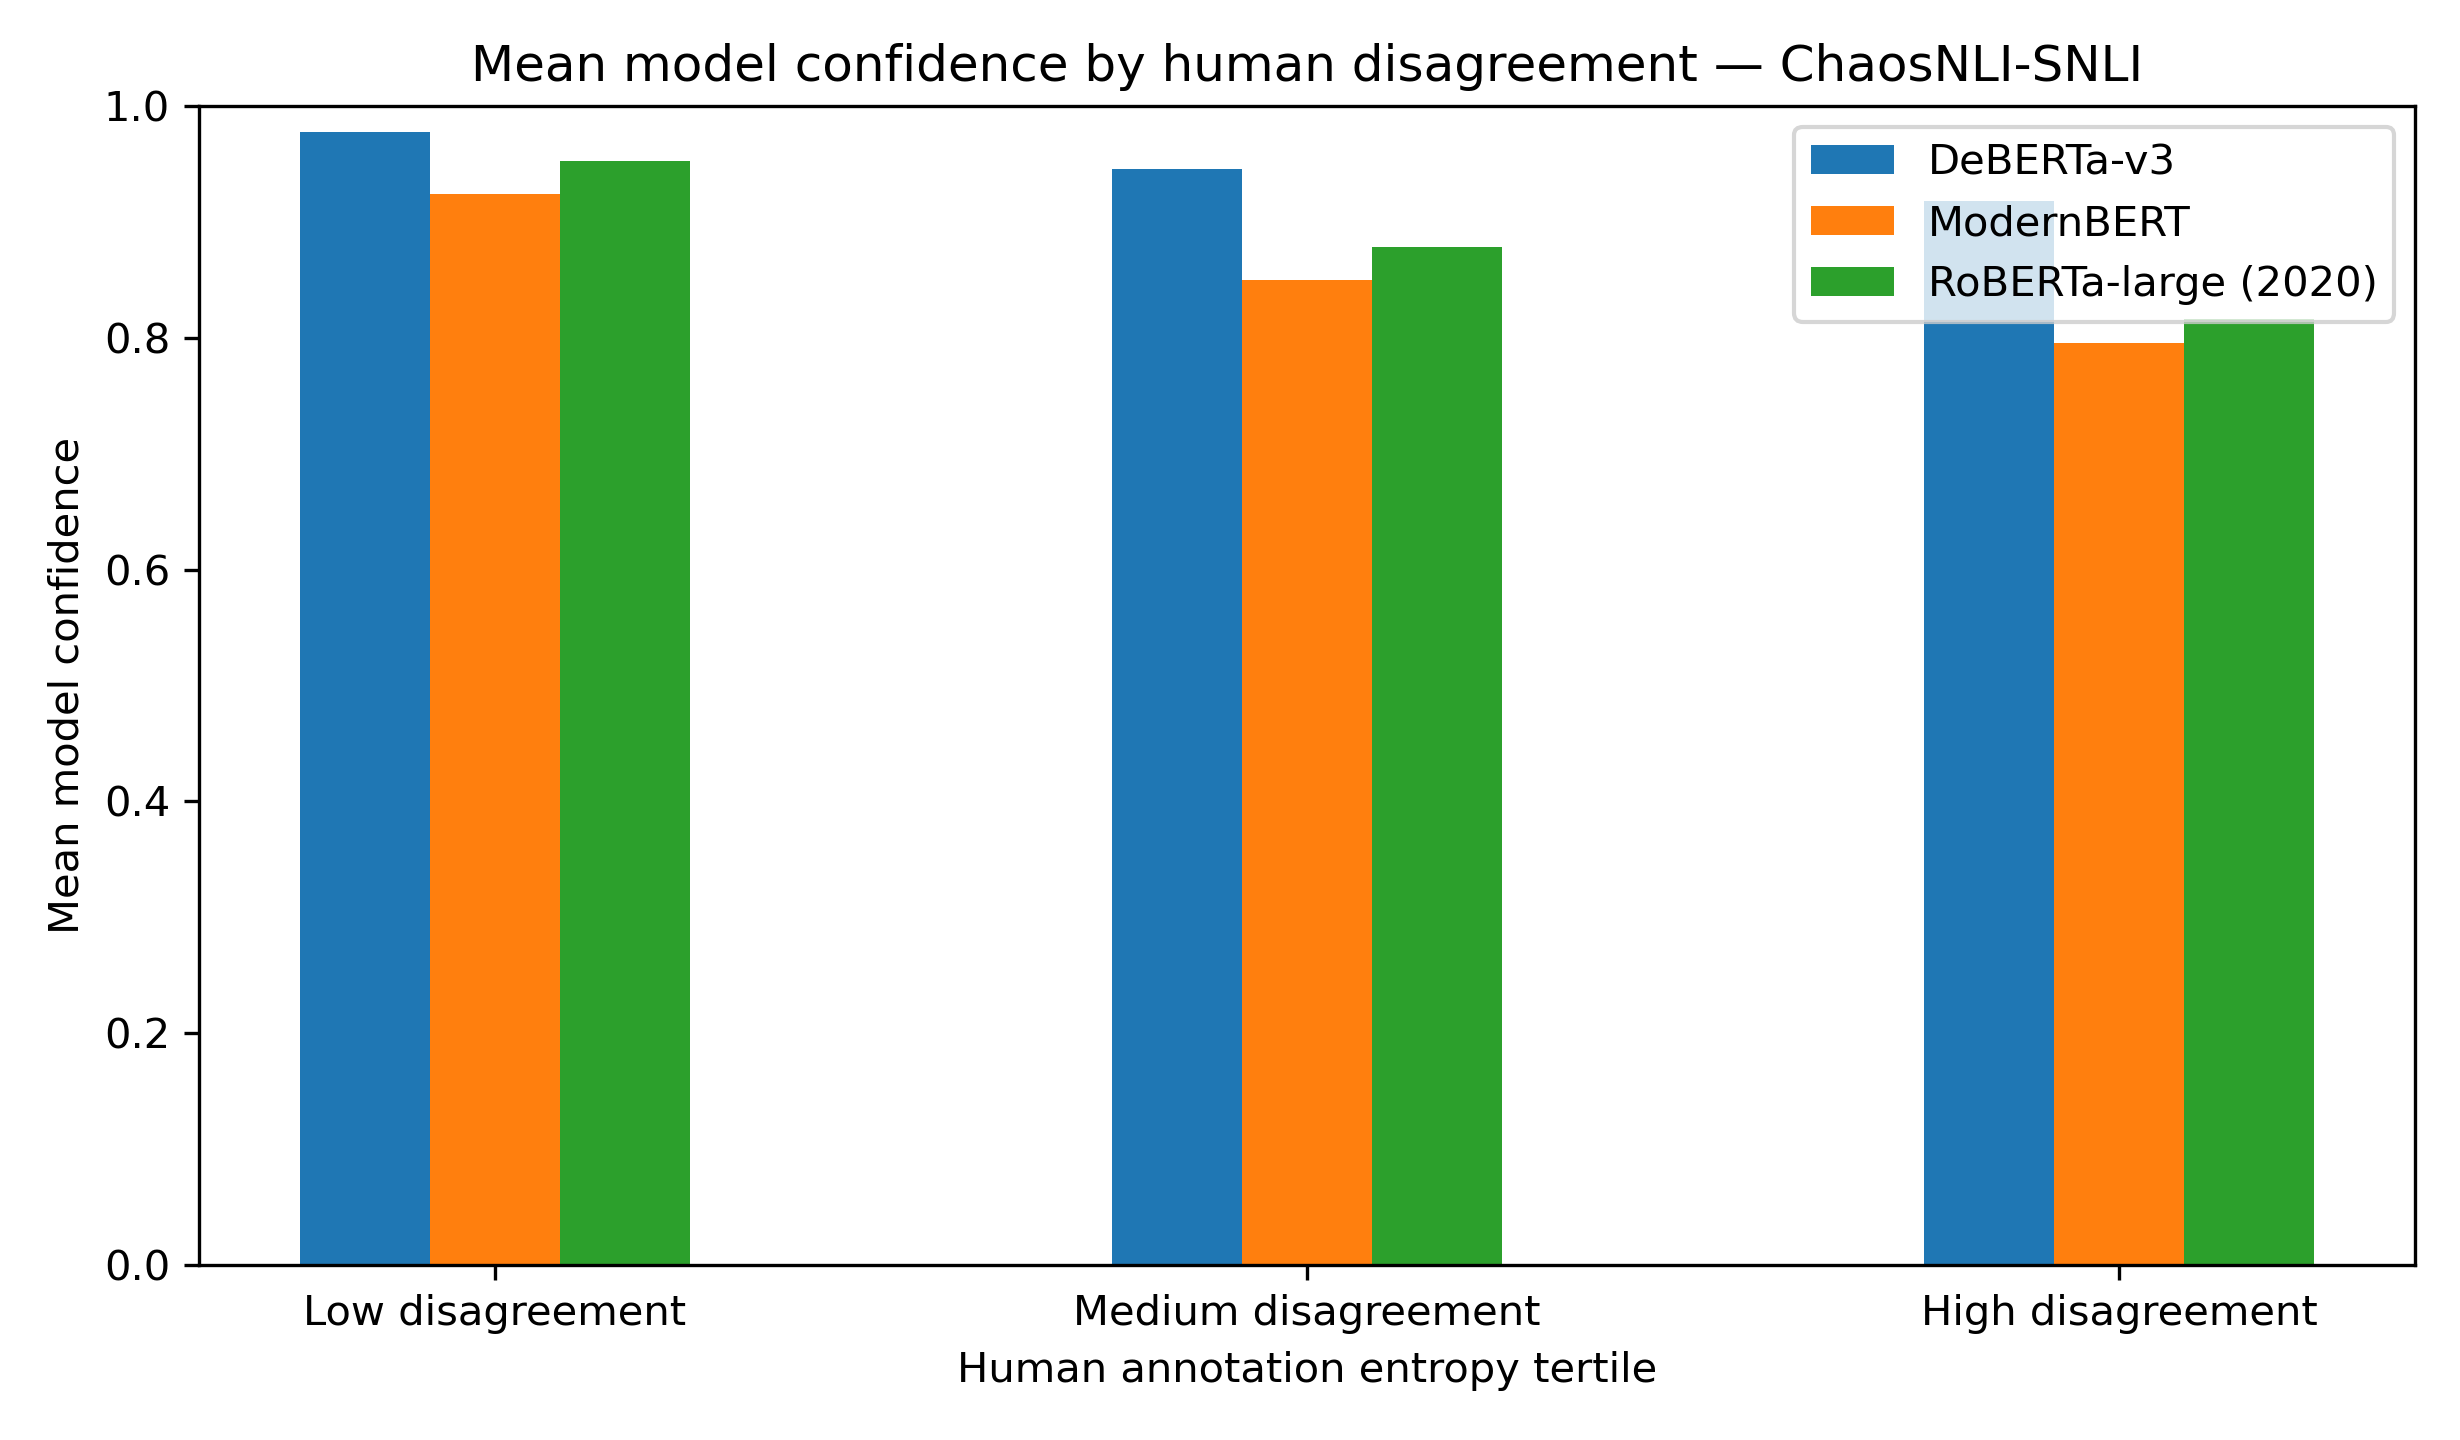
\includegraphics[width=0.85\textwidth]{snli_confidence_by_entropy.png}
\caption{Mean model confidence by human-disagreement tertile on ChaosNLI-SNLI.}
\label{fig:snli-conf}
\end{figure}

\begin{figure}[H]
\centering
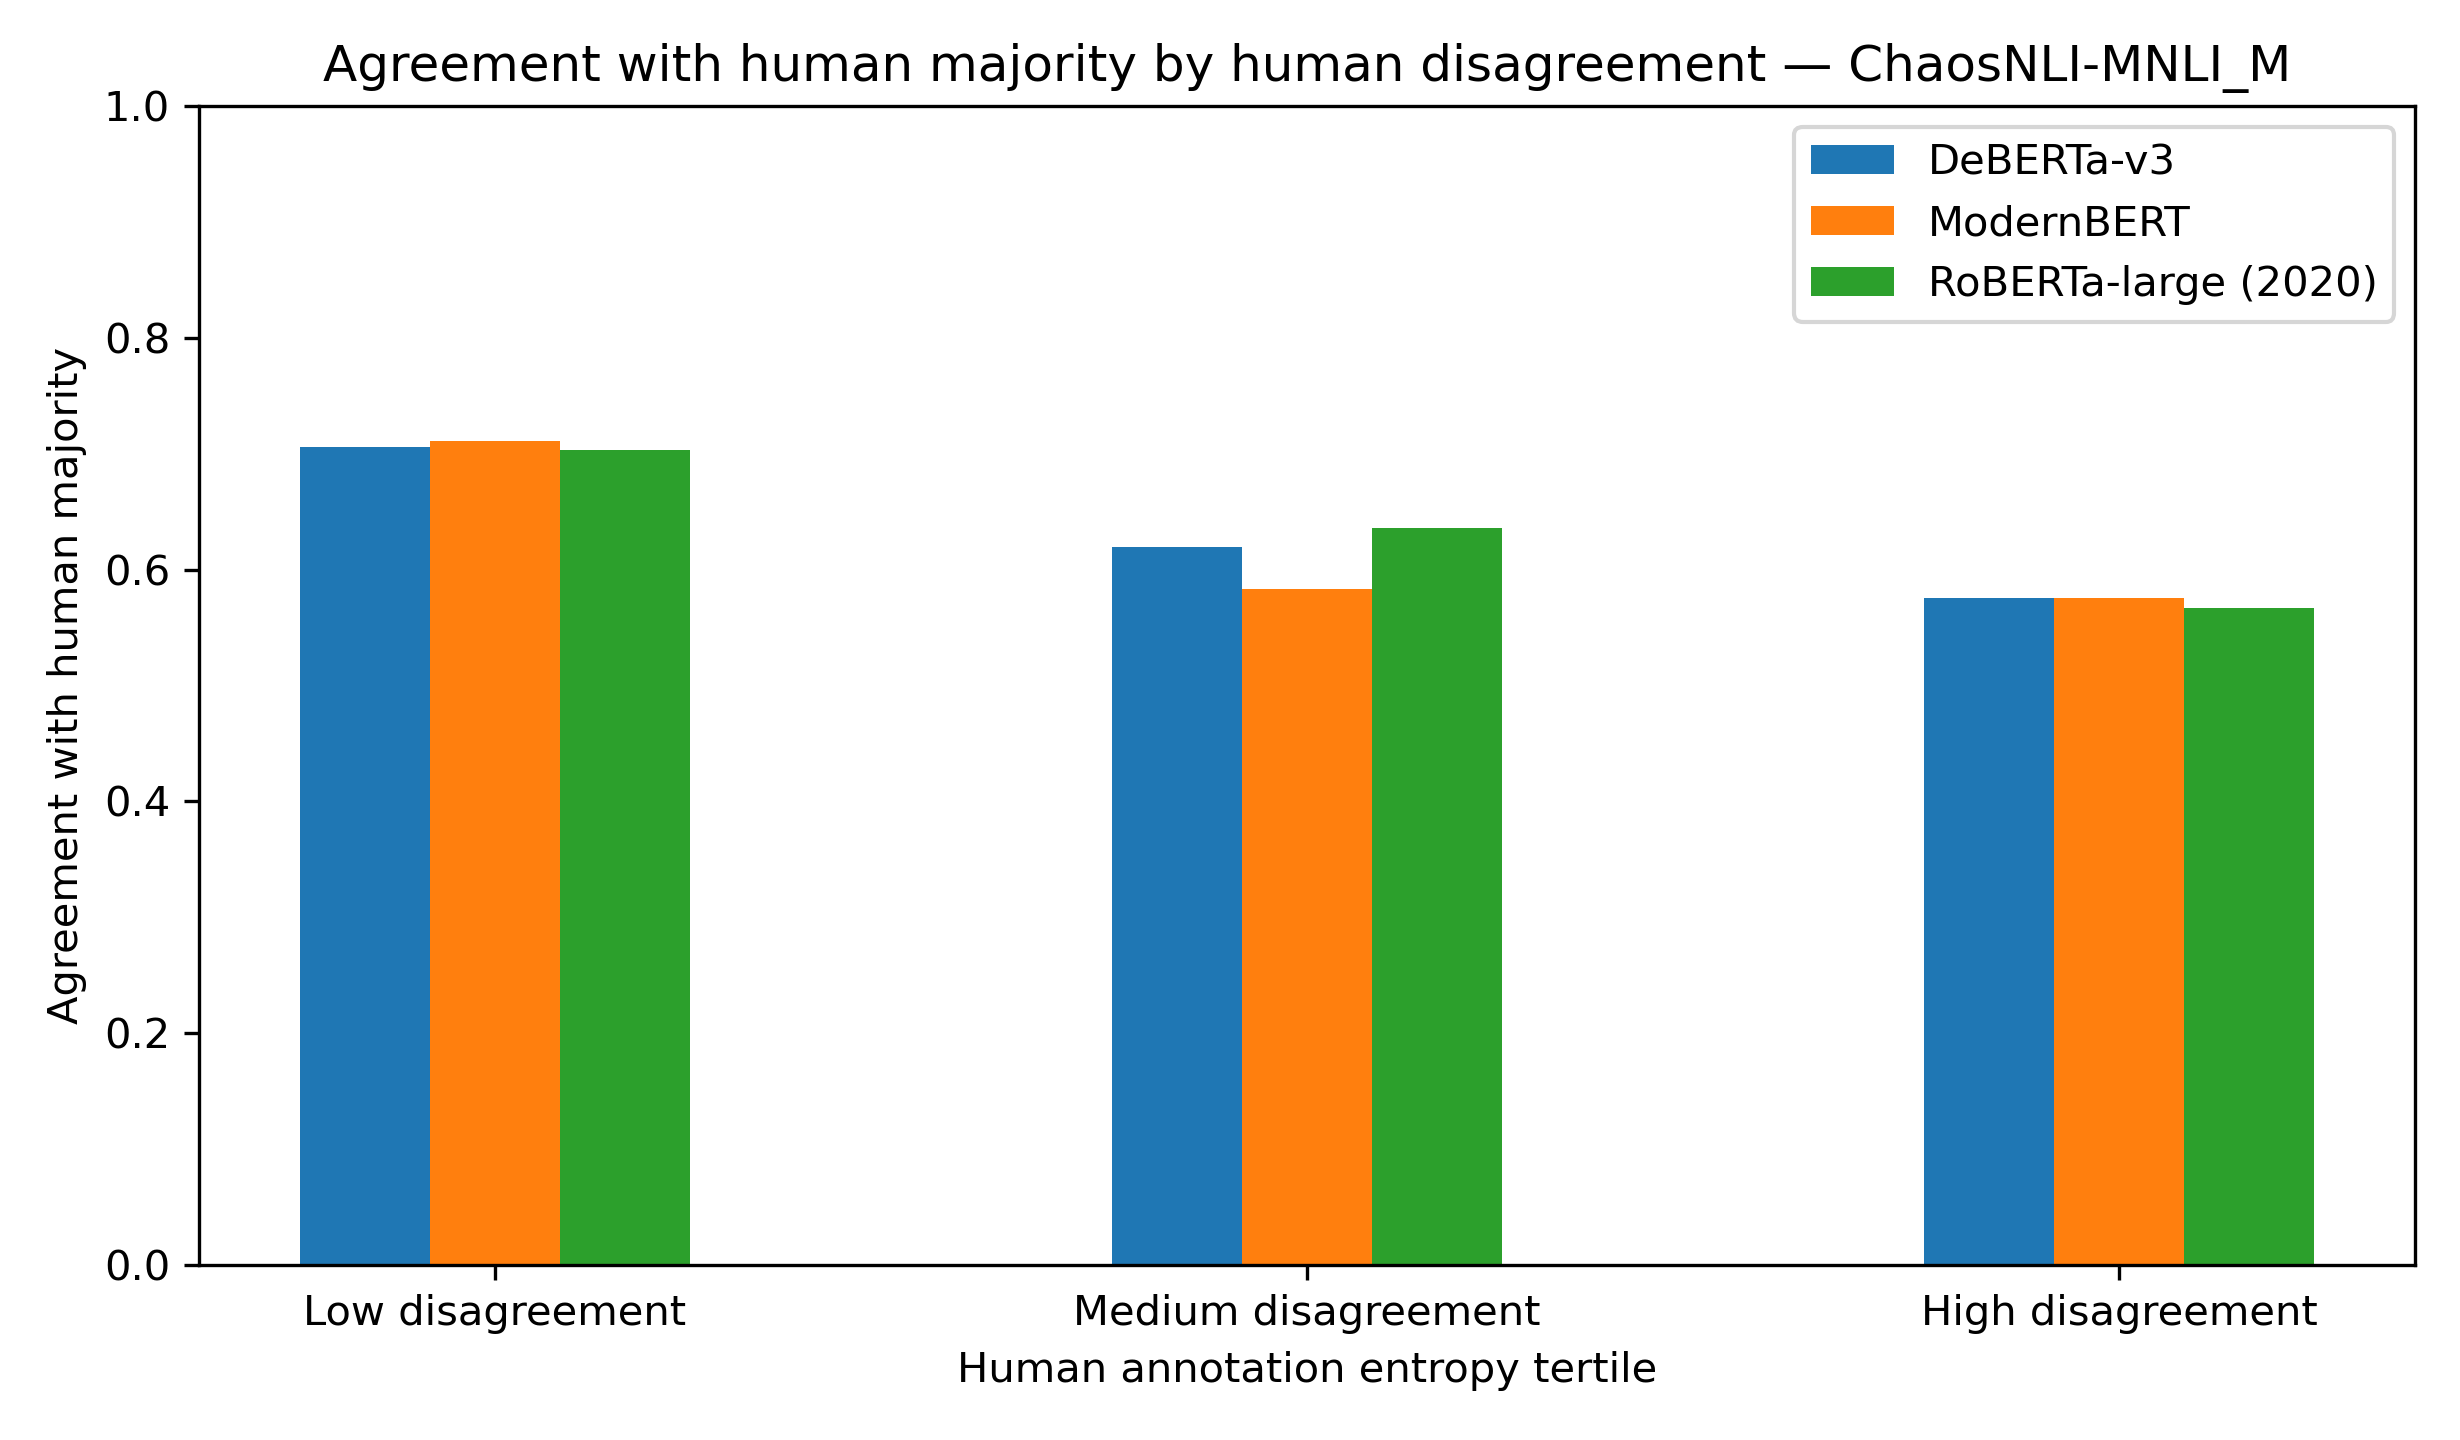
\includegraphics[width=0.85\textwidth]{mnli_m_new_acc_by_entropy.png}
\caption{Agreement with the 100-annotator majority by human-disagreement tertile on ChaosNLI-MNLI-matched.}
\label{fig:mnli-acc}
\end{figure}

\begin{figure}[H]
\centering
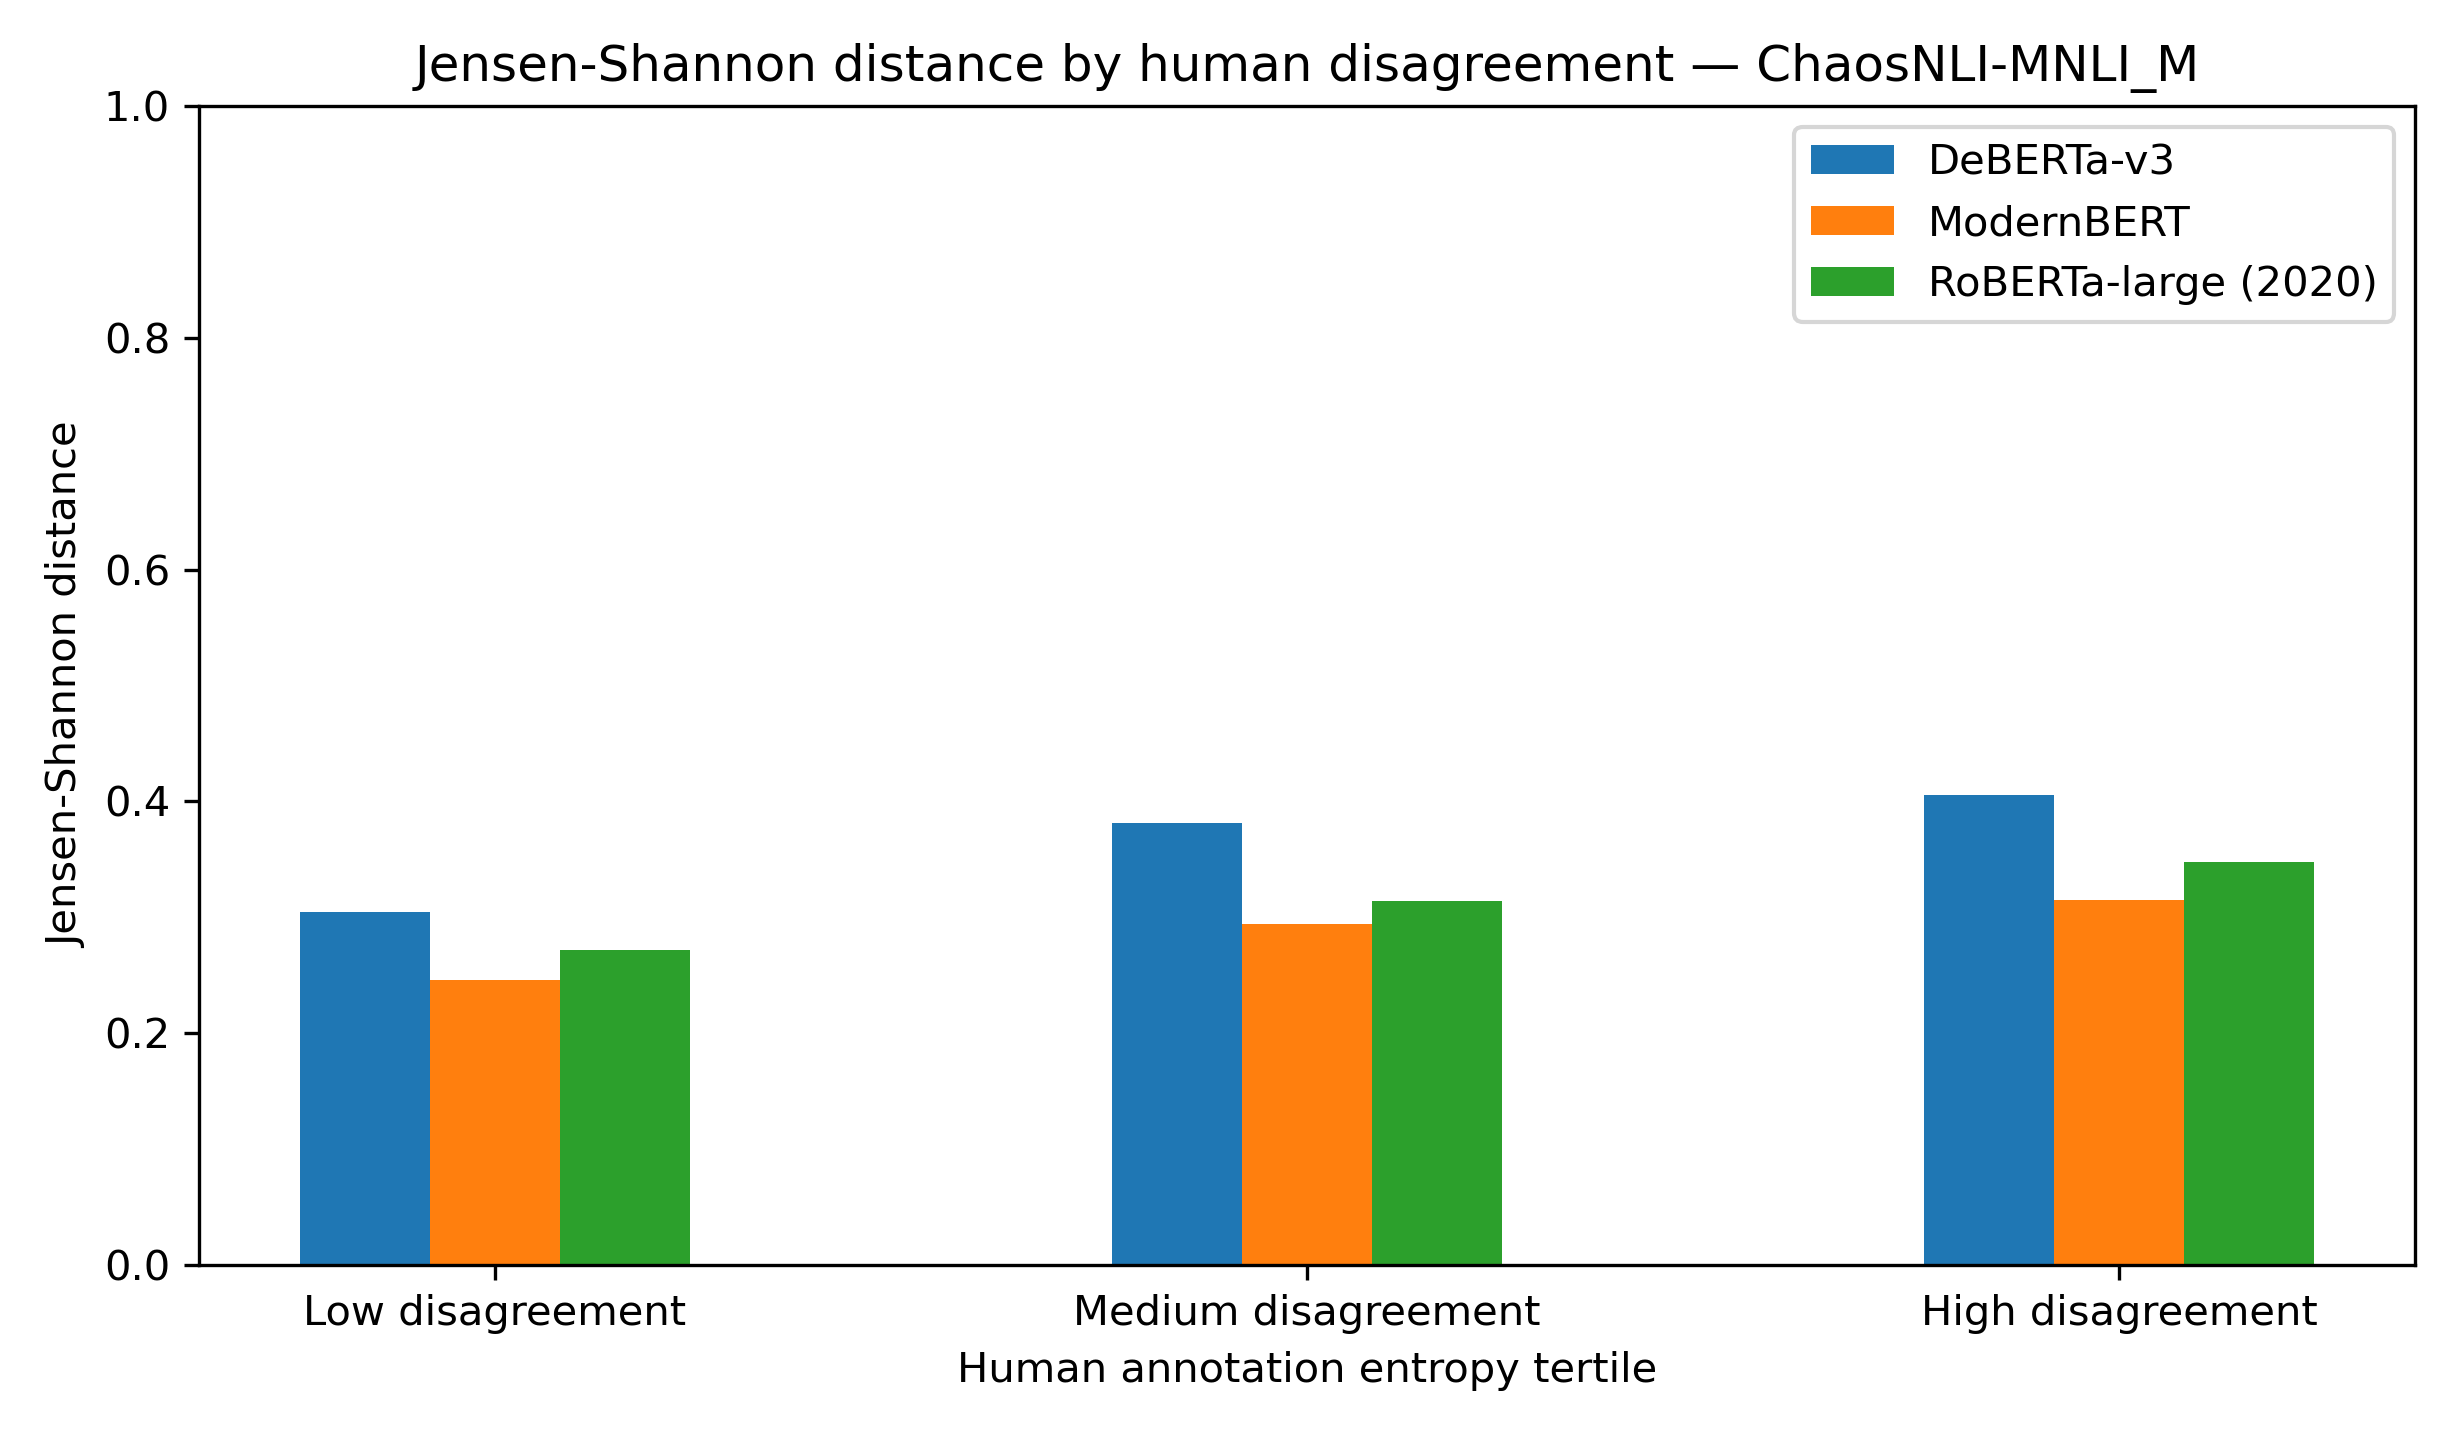
\includegraphics[width=0.85\textwidth]{mnli_m_jsd_by_entropy.png}
\caption{Jensen--Shannon distance by human-disagreement tertile on ChaosNLI-MNLI-matched.}
\label{fig:mnli-jsd}
\end{figure}

\begin{figure}[H]
\centering
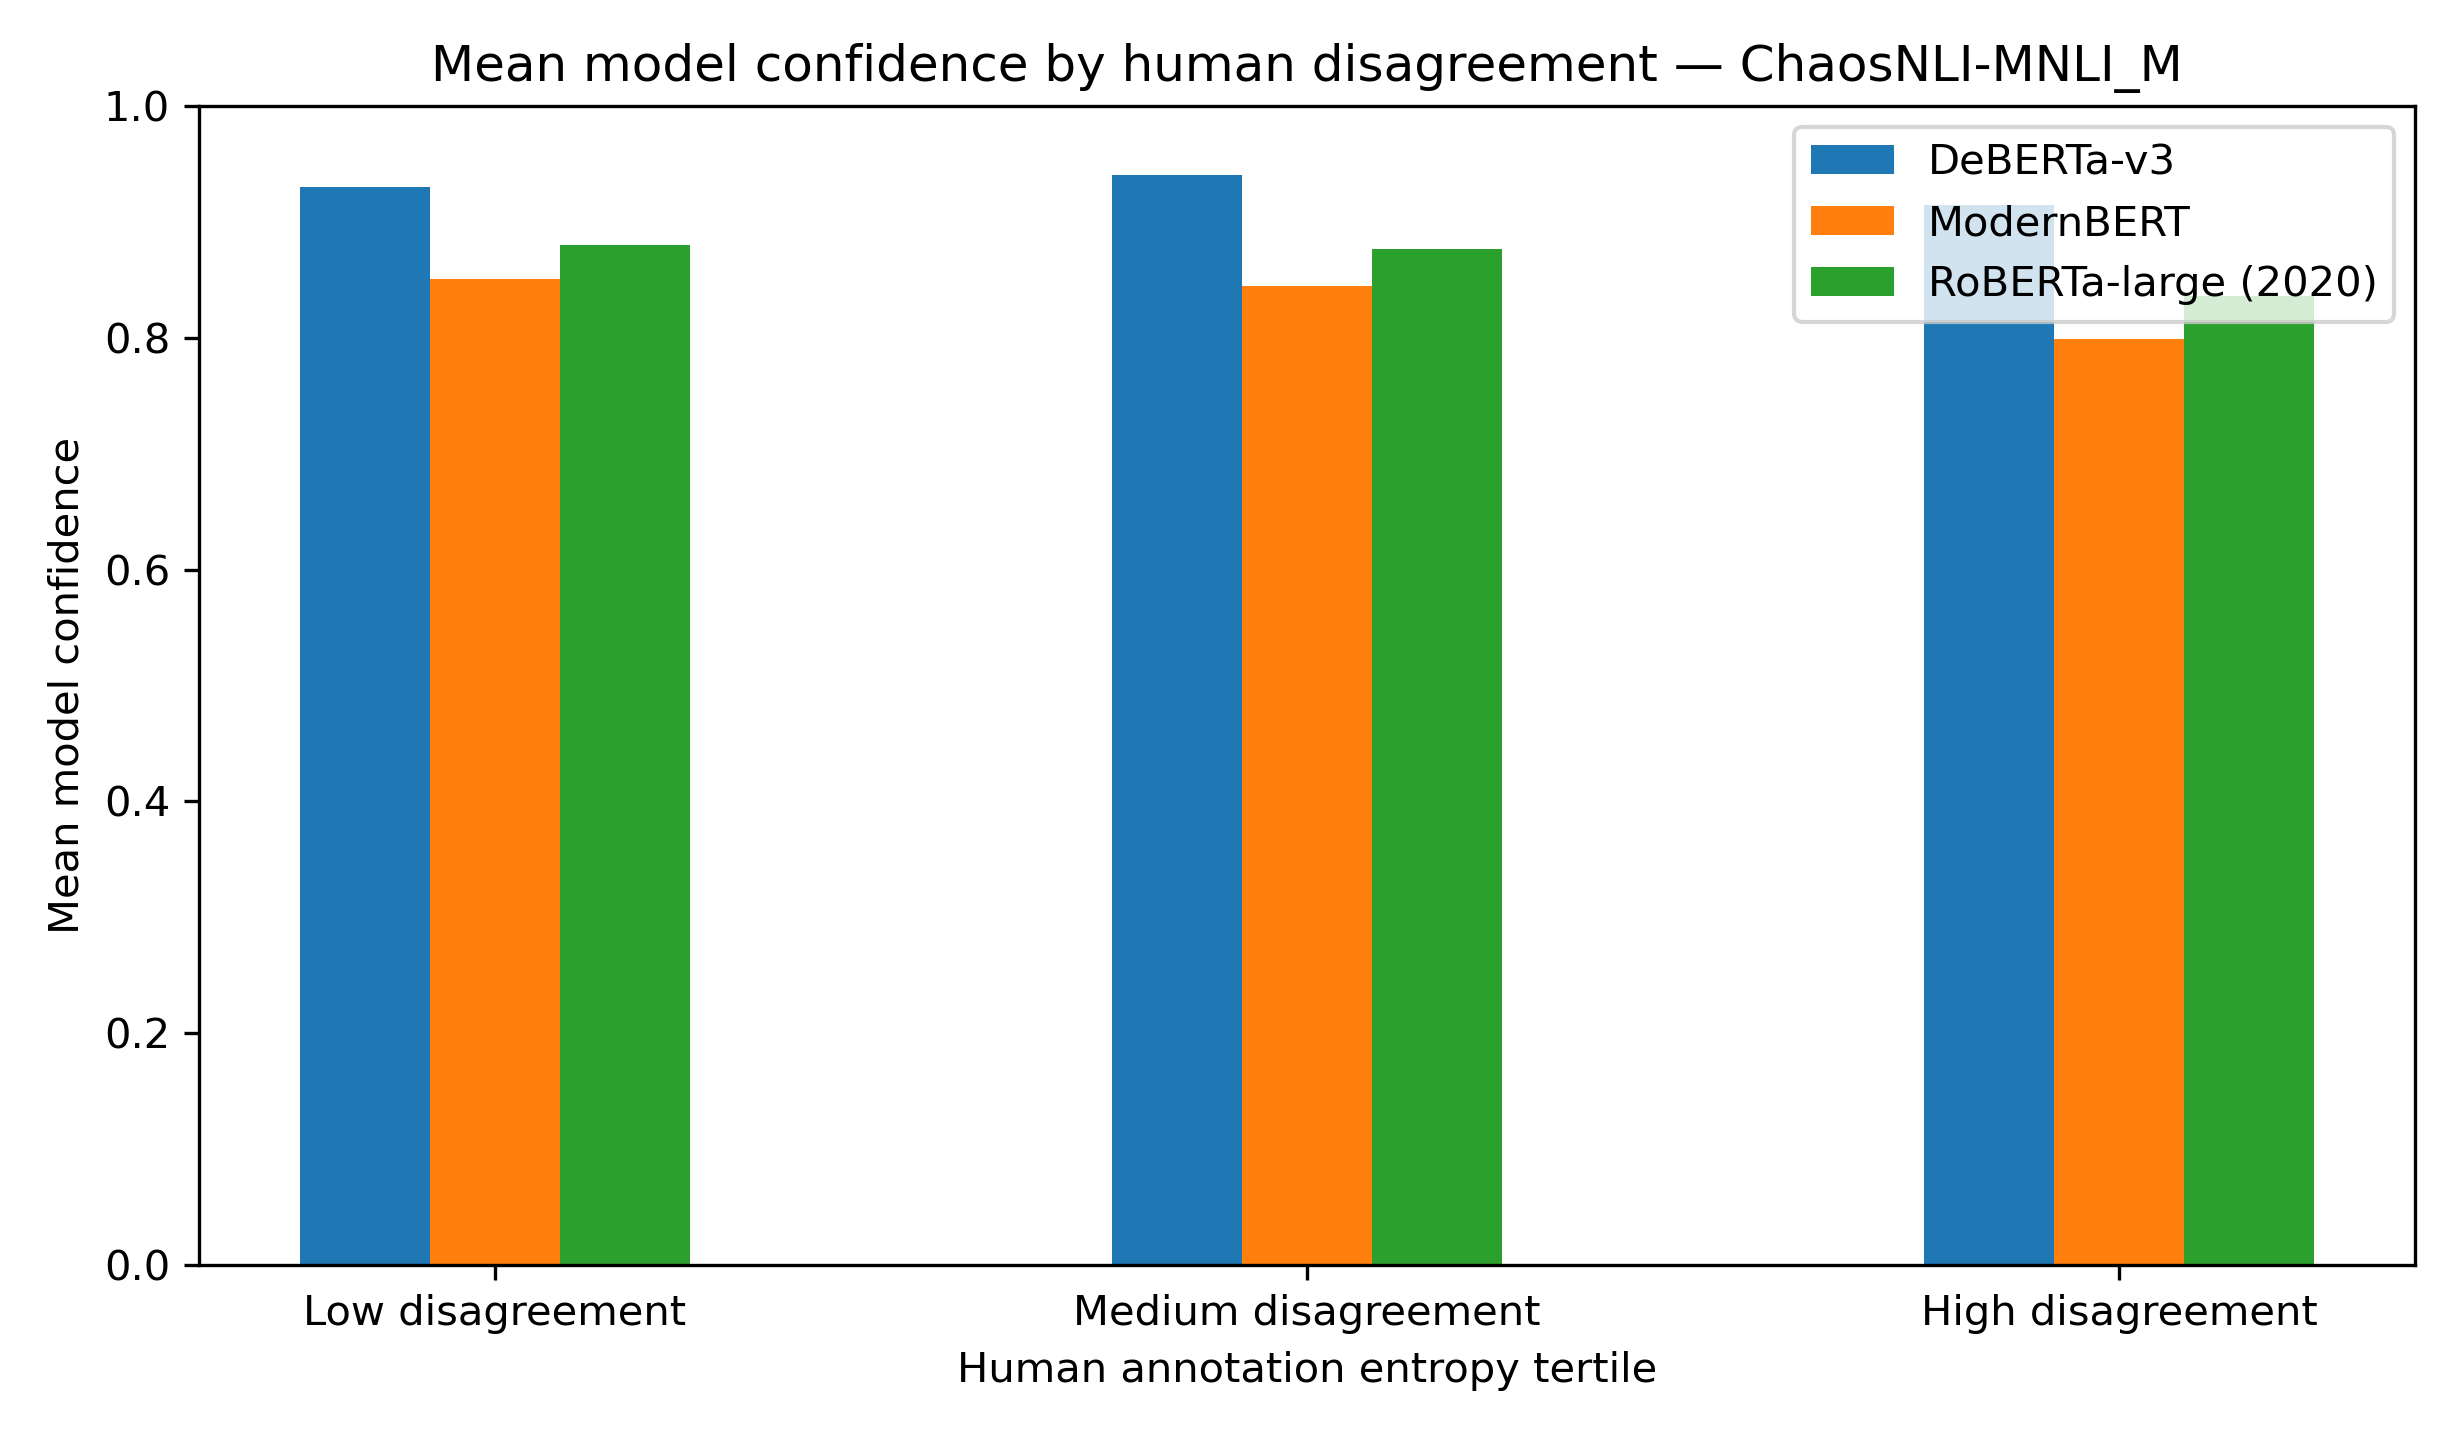
\includegraphics[width=0.85\textwidth]{mnli_m_confidence_by_entropy.png}
\caption{Mean model confidence by human-disagreement tertile on ChaosNLI-MNLI-matched.}
\label{fig:mnli-conf}
\end{figure}

\subsection{Agreement between the two modern models}

Table~\ref{tab:pair-snli} and Table~\ref{tab:pair-mnli} compare DeBERTa-v3 with ModernBERT. Figure~\ref{fig:consensus-snli} and Figure~\ref{fig:consensus-mnli} show the corresponding curves.

\begin{table}[H]
\centering
\small
\caption{DeBERTa-v3 and ModernBERT on ChaosNLI-SNLI, by entropy tertile.}
\label{tab:pair-snli}
\begin{tabular}{lccc}
\toprule
Tertile & Models agree & Both agree, both miss majority & Mean DeBERTa conf. \\
\midrule
Low & 0.913 & 0.018 & 0.978 \\
Medium & 0.794 & 0.095 & 0.946 \\
High & 0.679 & 0.224 & 0.918 \\
\bottomrule
\end{tabular}
\end{table}

\begin{table}[H]
\centering
\small
\caption{Same comparison on ChaosNLI-MNLI.}
\label{tab:pair-mnli}
\begin{tabular}{lccc}
\toprule
Tertile & Models agree & Both agree, both miss majority & Mean DeBERTa conf. \\
\midrule
Low & 0.803 & 0.191 & 0.930 \\
Medium & 0.788 & 0.291 & 0.941 \\
High & 0.705 & 0.263 & 0.915 \\
\bottomrule
\end{tabular}
\end{table}

On high-entropy SNLI the two models still pick the same label 68\% of the time. In 22\% of that tertile they agree with each other and not with the human majority. On MNLI they jointly miss the majority even in the low-entropy bin (19\%). Overall they agree on 80\% of SNLI and 77\% of MNLI. When they disagree, DeBERTa is slightly more often the one that matches the human majority (11\% vs.\ 9\% on SNLI; 12\% vs.\ 11\% on MNLI). They share MNLI, ANLI, WANLI, and LingNLI as training sources, and they share the same three-way label set. The shared errors look more like a common NLI convention than like two independent readings of the same ambiguity.

\begin{figure}[H]
\centering
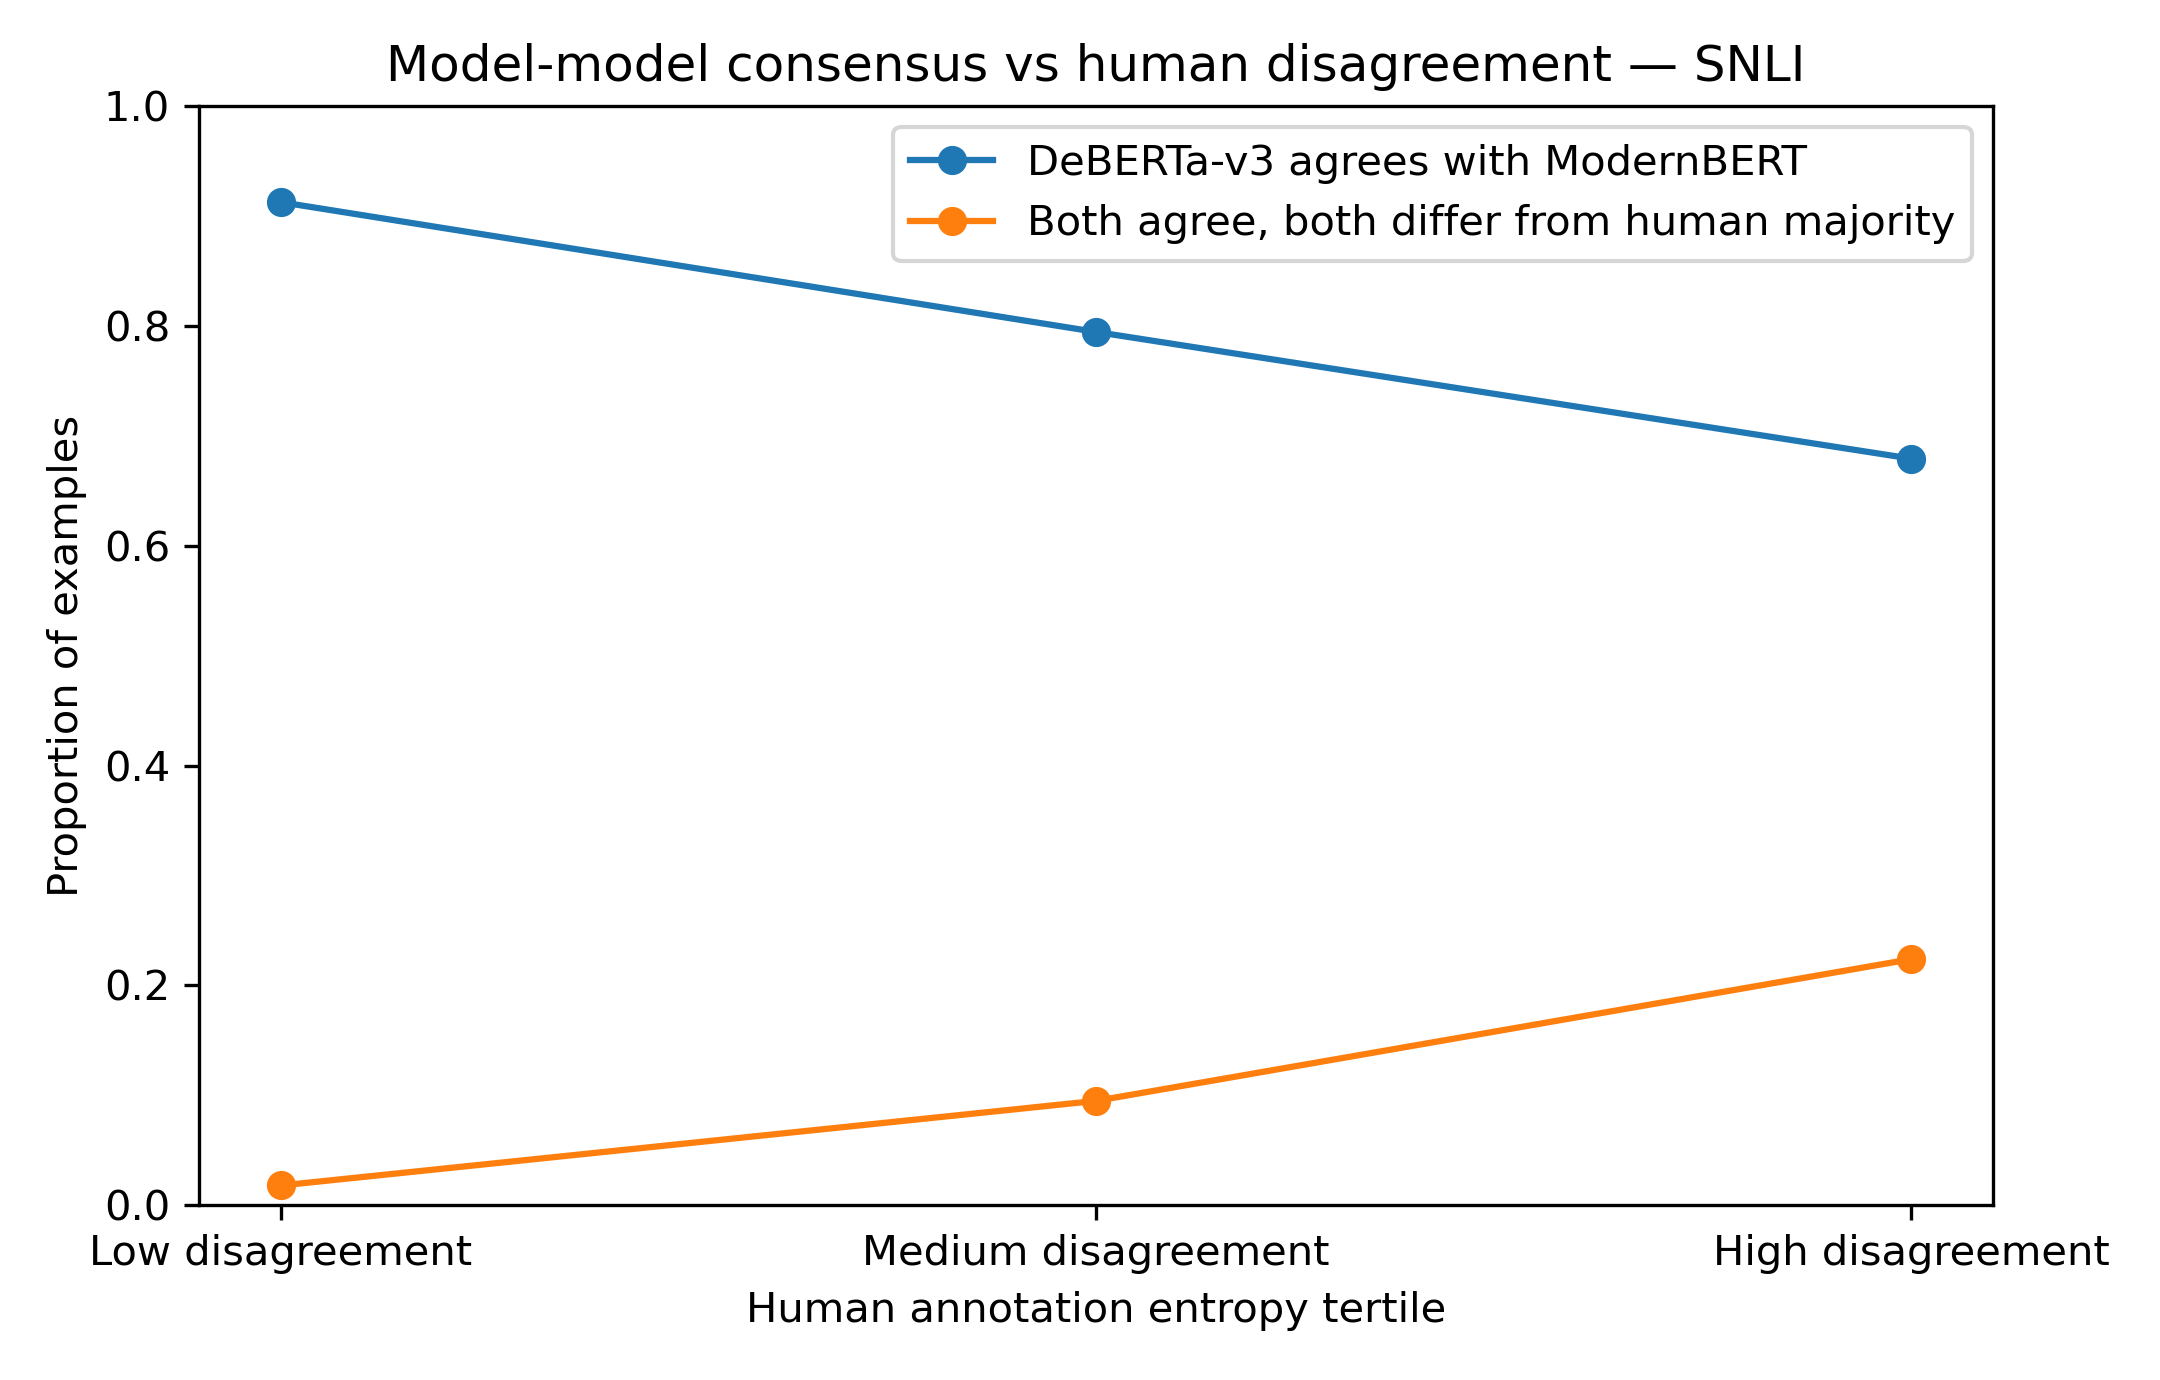
\includegraphics[width=0.85\textwidth]{snli_model_consensus_by_entropy.png}
\caption{Model--model consensus versus human disagreement on ChaosNLI-SNLI.}
\label{fig:consensus-snli}
\end{figure}

\begin{figure}[H]
\centering
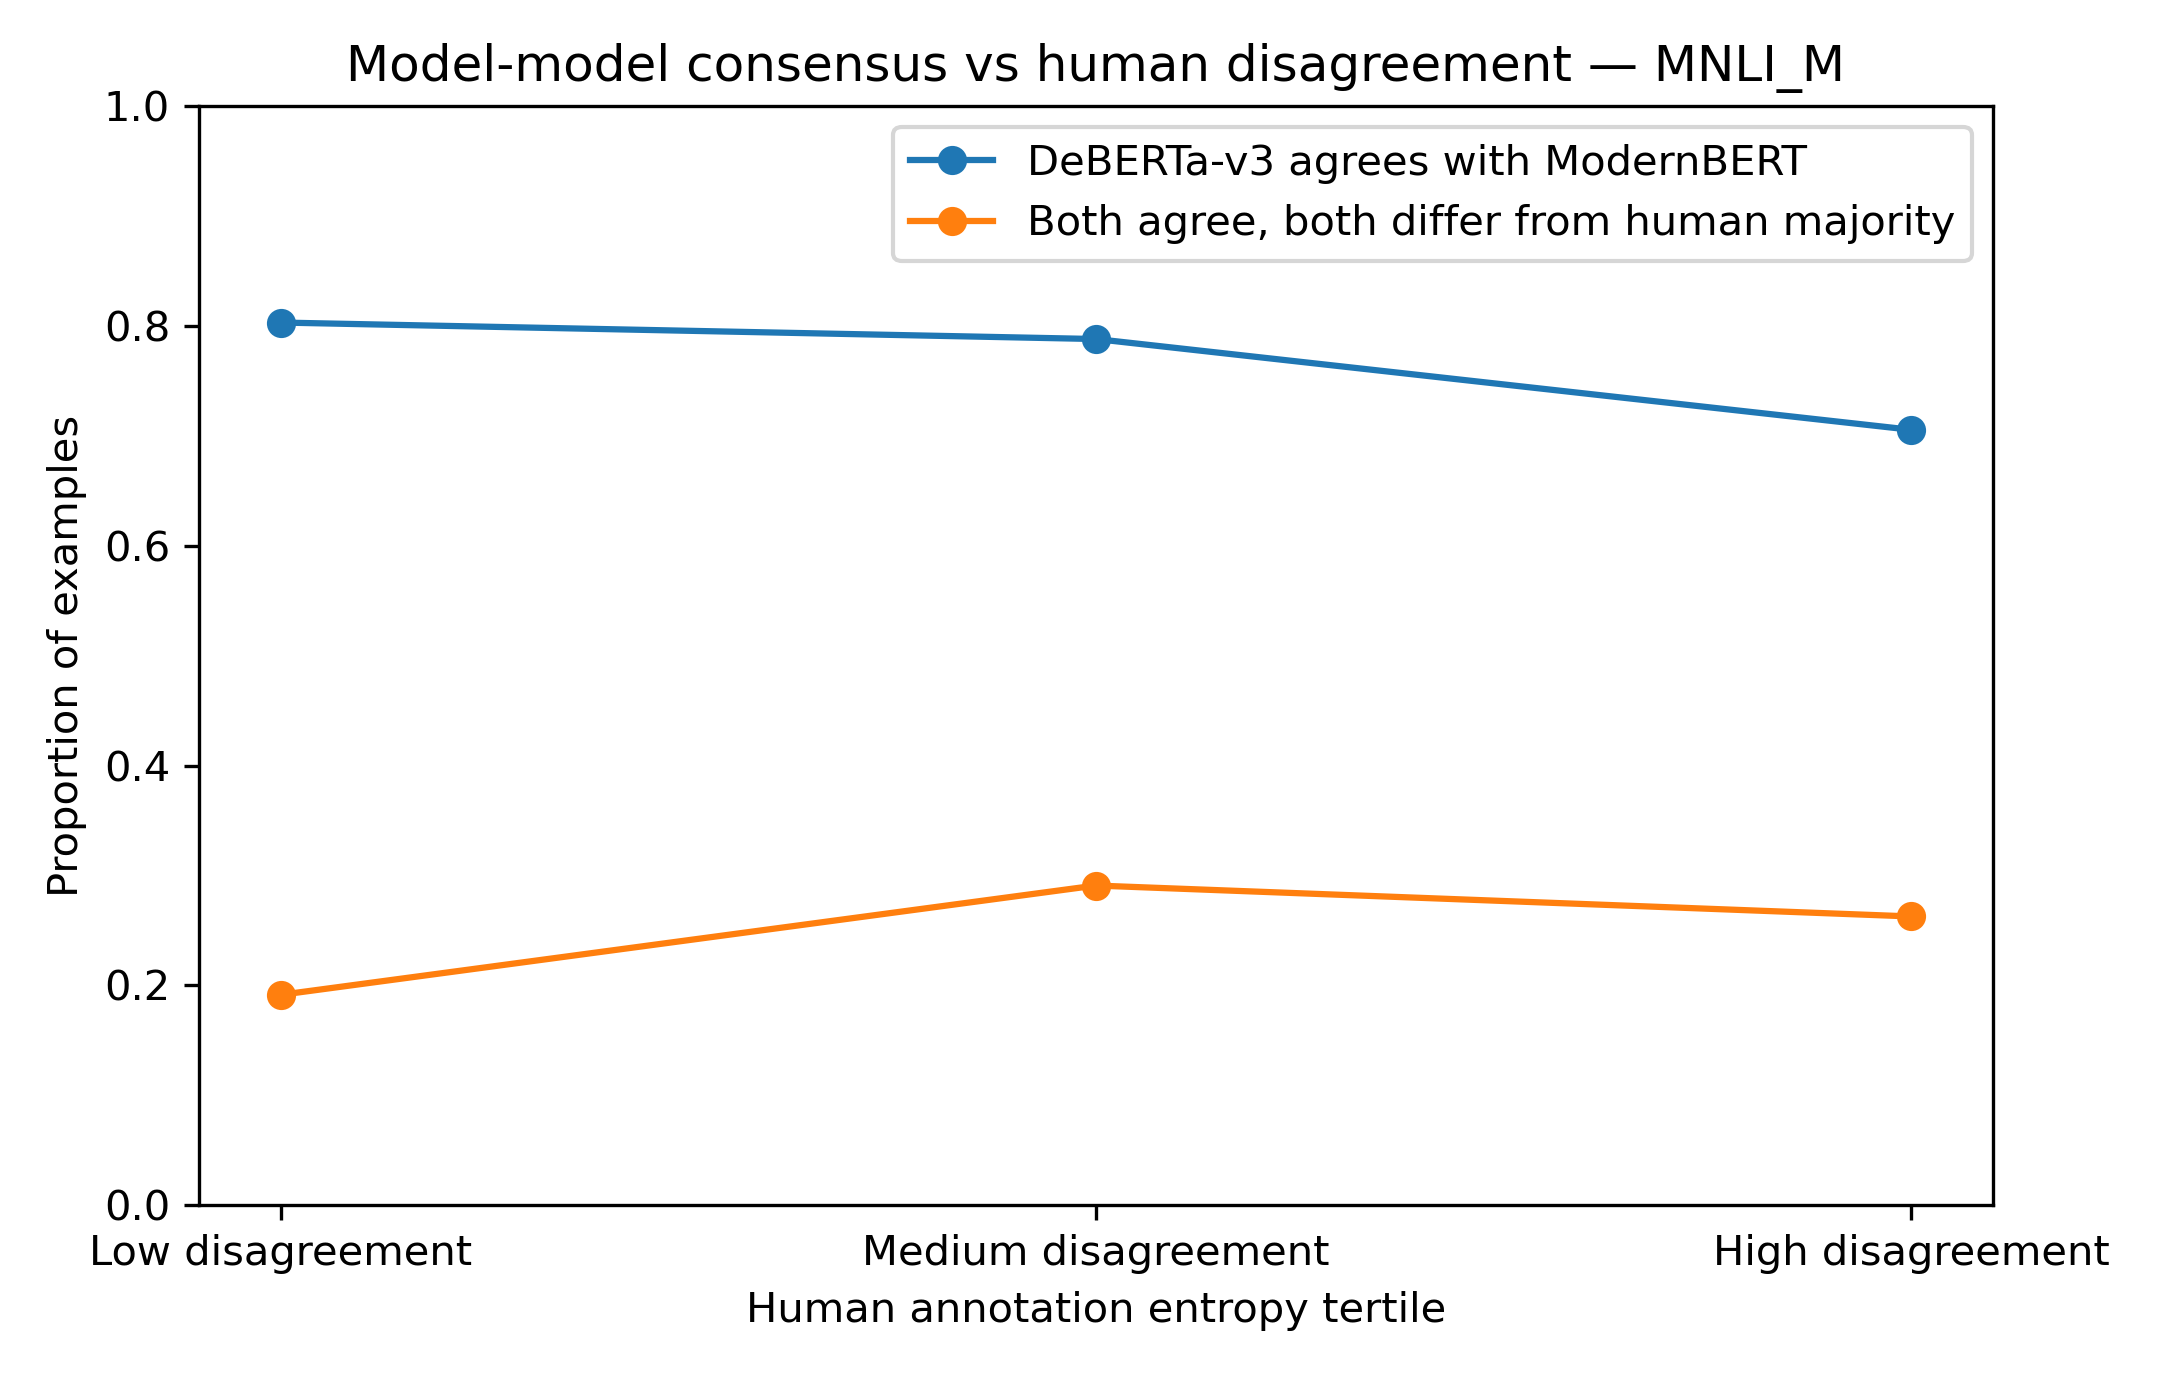
\includegraphics[width=0.85\textwidth]{mnli_m_model_consensus_by_entropy.png}
\caption{Model--model consensus versus human disagreement on ChaosNLI-MNLI-matched.}
\label{fig:consensus-mnli}
\end{figure}

\subsection{Temperature scaling}

Table~\ref{tab:temp} reports held-out temperature scaling.

\begin{table}[H]
\centering
\small
\caption{Temperature $T$ fit on a random half of each split, scored on the other half. Accuracy does not change.}
\label{tab:temp}
\begin{tabular}{lccc}
\toprule
Model / split & $T$ & Held-out JSD before / after & Held-out KL before / after \\
\midrule
DeBERTa SNLI & 2.75 & 0.276 / 0.187 & 0.848 / 0.195 \\
ModernBERT SNLI & 1.75 & 0.217 / 0.188 & 0.389 / 0.206 \\
DeBERTa MNLI & 4.50 & 0.358 / 0.206 & 1.430 / 0.211 \\
ModernBERT MNLI & 2.75 & 0.278 / 0.192 & 0.603 / 0.183 \\
\bottomrule
\end{tabular}
\end{table}

Temperature scaling reduces both JSD and KL divergence for all four model--dataset combinations. After softening, both models sit near JSD $0.19$. The largest change occurs for DeBERTa-v3 on MNLI, where JSD decreases from 0.358 to 0.206 and KL from 1.430 to 0.211. This setting also requires the highest temperature ($T=4.5$), indicating that the original probability distribution is particularly sharp. DeBERTa-v3 on SNLI requires a smaller but still substantial temperature of $T=2.75$. ModernBERT needs less softening, with $T=1.75$ on SNLI and $T=2.75$ on MNLI.

The entropy-matching experiment gives a similar result for DeBERTa-v3 on SNLI. Without using the labels, matching the mean model entropy to the mean human entropy gives $T=2.6$ and reduces JSD from 0.278 to 0.187. This is close to the JSD obtained with the temperature selected directly on the held-out JSD. The result suggests that the main difference between the original model distribution and the human distribution is partly related to prediction sharpness.

However, temperature scaling cannot reproduce the full structure of human disagreement. Because a single temperature is applied to every example, it only modulates overall prediction sharpness. Human disagreement varies from example to example. One item may have a distribution close to 50/50 between entailment and contradiction, while another may have a clear 95\% majority for entailment. Both examples are softened by the same temperature, even though their underlying uncertainty is different.

This limitation is important when interpreting the improvement in JSD and KL divergence. Temperature scaling can reduce excessive confidence and bring the model distributions closer to the human distributions, but it does not model item-specific disagreement. The experiment consequently suggests that part of the distribution mismatch comes from overly sharp predictions.

\subsection{Qualitative examples}

The selected examples reveal several recurring patterns in model--human disagreement.

\begin{itemize}[itemsep=0.5em, topsep=0.4em]

\item \textbf{Lexical mismatch that humans treat as scene description.}
One recurring pattern arises when the premise and hypothesis describe different actions or details of the same scene. The models can interpret these differences more strictly, while human annotators may treat them as compatible scene details.

\textbf{Premise:} ``A man in a dark suit talks with a middle-aged man and woman on a stage in front of a large logo of the letter `D' with the numeral five within it.''

\textbf{Hypothesis:} ``A couple of people are sitting in a room.''

\textbf{Human distribution:} entailment 18\%, neutral 58\%, contradiction 24\%.

\textbf{DeBERTa-v3 and ModernBERT:} contradiction at $\geq 98\%$ confidence.

Both models treat the difference between ``talks'' and ``sitting'' as a contradiction and assign almost all probability to contradiction. In contrast, the human distribution is dominated by neutral, suggesting that many annotators do not consider the two actions incompatible. A person can talk with others while sitting, so the hypothesis can be interpreted as a compatible description of the scene. This example illustrates how a lexical mismatch between the described actions can lead to a much sharper model prediction than the human distribution.

\item \textbf{Pragmatic inference versus strict entailment.}
A second pattern concerns cases where human annotators accept a plausible real-world inference as entailment, even though the hypothesis is not directly supported by the premise.

\textbf{Premise:} ``A boy in jeans, black t-shirt, and blue cap on a bike, leaps over steps.''

\textbf{Hypothesis:} ``A boy is practicing bike tricks.''

\textbf{Human distribution:} entailment 45\%, neutral 45\%, contradiction 10\%.

\textbf{DeBERTa-v3 and ModernBERT:} neutral at $\geq 95\%$ confidence.

The human distribution is almost evenly split between entailment and neutral, with a slight majority for entailment. Many annotators infer that the boy is practicing bike tricks, even though this is not explicitly stated in the premise. Both DeBERTa-v3 and ModernBERT instead predict neutral, matching the original SNLI dataset label. They favor a stricter interpretation and require more direct evidence for entailment.

\item \textbf{Near-paraphrase with split human labels.}
Human disagreement can also occur when the premise and hypothesis are very similar.

\textbf{Premise:} ``Closed on the Sabbath.''

\textbf{Hypothesis:} ``Sabbath is closed.''

\textbf{Human distribution:} entailment 37\%, neutral 24\%, contradiction 39\%.

\textbf{DeBERTa-v3 and ModernBERT:} entailment at approximately $98\%$ probability.

Both models produce highly concentrated distributions, with approximately 98\% of the probability on entailment. The premise and hypothesis are closely related in wording, which may explain why the two models arrive at the same prediction. At the same time, the human annotations are divided between entailment and contradiction. Word overlap is high, and neither softmax keeps mass on contradiction.

\item \textbf{Different representations of uncertainty.}
When the models disagree, ModernBERT is usually less peaked than DeBERTa-v3. Its probability is distributed more evenly across alternative labels, whereas DeBERTa-v3 often concentrates most of its probability on a single class.

\textbf{Premise:} ``A skateboard performs a trick off a quarter pipe.''

\textbf{Hypothesis:} ``A skateboard does a trick without a skateboarder.''

\textbf{Human distribution:} entailment 14\%, neutral 49\%, contradiction 37\%.

\textbf{DeBERTa-v3:} neutral at $99\%$ confidence, JSD $=0.45$.

\textbf{ModernBERT:} entailment 11\%, neutral 41\%, contradiction 48\%, JSD $=0.08$.

The premise describes a skateboard performing a trick. The hypothesis adds the detail that no skateboarder is present. The human annotators are largely split between neutral and contradiction. DeBERTa-v3 places almost all probability on neutral, while ModernBERT distributes its probability mainly between neutral and contradiction, with the highest probability on contradiction. ModernBERT has a much lower JSD and is closer to the human distribution, although contradiction is not the human majority label. This case shows that a less concentrated probability distribution can better represent human disagreement even when the predicted label does not match the human majority label.

\item \textbf{Unstated action on MNLI.}
MNLI errors are often extra inferences from written prose.

\textbf{Premise:} ``The judge gave vent to a faint murmur of disapprobation, and the prisoner in the dock leant forward angrily.''

\textbf{Hypothesis:} ``The judge ordered the court to be silent.''

\textbf{Human distribution:} entailment 24\%, neutral 45\%, contradiction 31\%.

\textbf{DeBERTa-v3 and ModernBERT:} contradiction at $\geq 99\%$ confidence.

The hypothesis adds an order that is not in the premise. Many annotators still called the pair neutral rather than a hard contradiction. Both models treat the extra action as incompatible with the premise.

\item \textbf{Original MNLI label versus 100 annotators.}
The last pattern matches the mismatch analysis in Section~\ref{sec:errors}.

\textbf{Premise:} ``so we've been out here well really in the house since December and we've been uh planting flowers that we could never plant in San Antonio uh''

\textbf{Hypothesis:} ``We planted lots of different flowers in San Antonio.''

\textbf{Human distribution:} entailment 18\%, neutral 53\%, contradiction 29\%.

\textbf{Original MNLI label:} contradiction.

\textbf{DeBERTa-v3 and ModernBERT:} contradiction at $\geq 91\%$ confidence.

The 100-annotator majority is neutral. Both models keep the older MNLI label. This is the MNLI mismatch pattern: the checkpoints were trained on MNLI and still often follow that convention when 100 annotators vote the other way.

\end{itemize}

The qualitative examples cover several forms of model--human disagreement. DeBERTa-v3 and ModernBERT can remain highly confident even with variation in the human annotations. They can also apply stricter interpretations than some annotators. On SNLI the typical miss is a lexical clash that humans treat as a scene. On MNLI the typical miss is a hypothesis that adds a small inference, which the models often send to contradiction or, when the original dataset label was already conservative, keep as that older label. In addition, the two models differ in how they represent alternative labels. These observations support the use of distributional measures alongside majority-label accuracy when evaluating model alignment with human judgments.

\section{Discussion}

Table~\ref{tab:strengths} is a compact view of the same results.

\begin{table}[H]
\centering
\small
\caption{Where each checkpoint is strong or weak on ChaosNLI.}
\label{tab:strengths}
\begin{tabular}{p{2.4cm}p{5.4cm}p{5.4cm}}
\toprule
 & DeBERTa-v3 & ModernBERT \\
\midrule
SNLI strength & Highest new accuracy (0.793); low-entropy bin 94.8\%; prefers the 100-annotator majority when it disagrees with the old SNLI label & Best JSD and KL; less peaked softmax (mean conf.\ 0.86) \\
SNLI weakness & Worst JSD/KL; mean confidence 0.95 & New accuracy below RoBERTa (0.768); more false contradiction \\
MNLI strength & Best old accuracy (0.695); high contradiction recall (0.80) & Best JSD (0.285) and KL (0.638) among all models we compare \\
MNLI weakness & Worst KL (1.465); confidence vs.\ human entropy $\rho=-0.05$; follows old MNLI labels when they disagree with the new majority & Same entailment collapse (recall 0.52); false-neutral rate 0.23 \\
High disagreement & About 61\% SNLI / 58\% MNLI new accuracy; still $\ge$91\% mean confidence & About 60\% SNLI / 58\% MNLI; confidence drops more (0.80 on high-entropy SNLI) \\
\bottomrule
\end{tabular}
\end{table}

Both checkpoints are 3-way classifiers trained with cross-entropy on one gold label. That loss is minimized by putting almost all probability on one class. ChaosNLI scores the full softmax against a 100-person distribution that is often spread across two labels. If humans put 20\% on contradiction and the model puts 0.1\%, KL becomes large even when the model's top label is the majority. DeBERTa-v3 can therefore be the strongest majority classifier in the SNLI table and the weakest distribution model at the same time. Nie et al.\ already saw a version of this with DistilBERT. The same split is more extreme on the Laurer checkpoint.

DeBERTa-v3 was trained on a large hard-label mix (about 885k pairs). Extra one-hot NLI data helps the ranking of the majority class and also trains very certain logits. Mean SNLI confidence is 0.95. On MNLI, confidence barely moves with human entropy. Temperature scaling is a direct test of that account: $T=2.75$ on SNLI and $T=4.5$ on MNLI cut JSD roughly in half without changing any predicted label. The ranking was often already right. The distribution was too sharp.

ModernBERT's mix is broader, with many NLI-format tasks under multi-task fine-tuning. It never becomes as peaked: mean SNLI confidence 0.86, mean model entropy 0.53 bits rather than 0.21. A softer distribution is closer to a spread-out human distribution, which improves JSD and KL even when the argmax is not better. WANLI and related sets are built from worker disagreement, so the model sees more label variation than a classic MNLI-only encoder, still under hard labels. That is not the same as learning the ChaosNLI 100-way target, but it can limit collapse onto a single convention. On the skateboard example, ModernBERT does not resolve the ambiguity better in any deep sense. It is less willing to zero out the other plausible class.

High-entropy items look underspecified rather than merely difficult: verb mismatch, extra inferred detail, near-paraphrase. A stronger encoder can learn the majority convention on low-entropy items (DeBERTa reaches 94.8\% there on SNLI). Hard-label training has no target of the form ``45\% of people will call this entailment,'' so the high-disagreement slice stays near the 2020 numbers.

The two modern models agree with each other more than they agree with divided humans because they share a label space and overlapping NLI sources. They learn similar heuristics: lexical overlap, conservative neutrality on extra details, sharp contradiction on mismatched verbs. Humans split for other reasons. That looks like a shared training convention, not two systems recovering the same human uncertainty.

Strengths are easy to list from the same tables. DeBERTa-v3 is the better majority-label model on SNLI, including the low-entropy bin (94.8\%). It is also the better old-label model on MNLI, which is expected: MNLI was in its training mix and SNLI was not. ModernBERT is the better distribution model on both splits. Its SNLI JSD (0.214) beats BART-large, and its MNLI JSD (0.285) is the only score in our table that moves clearly below the 2020 cluster. If the question is who hits the ChaosNLI majority on captions, DeBERTa wins. If the question is whose softmax looks more like 100 annotators, ModernBERT wins.

The SNLI-to-MNLI drop is a generalization failure of a specific kind. Accuracy on majority entailment collapses; contradiction does not. Both models respond to MNLI disagreement by dumping probability on neutral. That is not the same as matching the human distribution, because the MNLI majority is often entailment. It is closer to a conservative NLI policy: if the hypothesis is not a near-paraphrase, call it neutral. Temperature scaling can fix sharpness. It cannot invent a different policy for those items.

Lee et al.\ already showed that moving from RoBERTa to GPT-3 does not fix ChaosNLI JSD. ModernBERT is a smaller change: still an encoder, still trained as a classifier, but with a broader multi-task mix and a less peaked softmax. It does beat the 2020 RoBERTa JSD numbers. That is a modest, encoder-side update to Lee's result, not a claim that the disagreement problem is solved. DeBERTa-v3 is the other side of the same update: more NLI data and a better majority classifier, with worse JSD than BERT-large.

We did not retrain DeBERTa on ModernBERT's mix, or the reverse. The account above is based on the metrics, the model cards, and the temperature results, not on a causal ablation. It is consistent with \cite{nie2020chaosnli,meissner2021capturing,baan2022stop,pavlick2019inherent}.

\section{Limitations}

We evaluate frozen checkpoints. Soft-label training on ChaosNLI is already known to help \cite{zhou2022distributed} and is a different experiment. We omit $\alpha$NLI. Temperature scaling uses a random split of ChaosNLI itself, so it is a diagnostic rather than a calibrator one would ship. A single global temperature only adjusts prediction sharpness and cannot capture item-specific human disagreement. Because we stored softmax probabilities rather than logits, the temperature search is run on $\log p$, which is an approximation to the original logits.

JSD and KL follow the official ChaosNLI implementation so that 2020 rows remain comparable. The discussion of training data is inferred from public model cards, not from a controlled re-train.

The evaluation is limited to two recent NLI checkpoints and two ChaosNLI subsets, so the findings may not generalize to other models or datasets. Entropy tertiles are a convenience split, not a claim that disagreement has three natural types. The qualitative analysis is based on a small number of targeted examples. The patterns here are not exhaustive and do not form a systematic taxonomy of model--human disagreement.

\section{Conclusion}

We scored two later NLI checkpoints on ChaosNLI with the original JSD, KL, old accuracy, and new accuracy protocol. DeBERTa-v3 improves majority-label accuracy on SNLI and old accuracy on MNLI, and it is worse than the 2020 encoders on distribution match. ModernBERT improves JSD and KL, including a clear MNLI JSD gain, without beating RoBERTa-large on majority accuracy. High-disagreement accuracy stays near 60\%. The two models often pick the same label when annotators do not. On MNLI both lose about half of majority-entailment items to neutral, and when the original MNLI label disagrees with the 100-annotator majority they tend to keep the original label. Temperature scaling shows that much of the JSD gap is excess confidence. Encoder NLI progress since 2020 did not, by itself, close the disagreement problem posed by ChaosNLI.

\section*{Acknowledgements}

ChaosNLI data and the 2020 baseline predictions are from Nie, Zhou, and Bansal. The two checkpoints are public Hugging Face models from Laurer et al.\ and from tasksource. This report was prepared as a seminar project.

\appendix
\section{Reproducibility}

Predictions, metrics, and plots are under \texttt{results/}. From the project root:

\begin{verbatim}
python src/evaluate_models.py deberta snli
python src/evaluate_models.py deberta mnli_m
python src/evaluate_models.py modernbert snli
python src/evaluate_models.py modernbert mnli_m
python src/analyze_findings.py
\end{verbatim}

The four evaluation jobs write JSON prediction files. The analysis script then recomputes the official ChaosNLI metrics against the 2020 baselines, builds the entropy-bin tables and plots, runs temperature scaling, and writes \path{results/findings_summary.json}. The report source is \path{report/nli_disagreement.tex}. Compile with \texttt{pdflatex} from the \texttt{report/} directory and copy the PDF to \texttt{REPORT.pdf} in the project root.

\bibliographystyle{plain}
\begin{thebibliography}{99}

\bibitem{baan2022stop}
Joris Baan, Wilker Aziz, Barbara Plank, and Raquel Fern\'andez.
\newblock Stop measuring calibration when humans disagree.
\newblock In {\em Proceedings of EMNLP}, 2022.

\bibitem{bowman2015snli}
Samuel~R. Bowman, Gabor Angeli, Christopher Potts, and Christopher~D. Manning.
\newblock A large annotated corpus for learning natural language inference.
\newblock In {\em Proceedings of EMNLP}, 2015.

\bibitem{he2023debertav3}
Pengcheng He, Jianfeng Gao, and Weizhu Chen.
\newblock DeBERTaV3: Improving DeBERTa using ELECTRA-style pre-training with gradient-disentangled embedding sharing.
\newblock In {\em Proceedings of ICLR}, 2023.

\bibitem{laurer2024less}
Moritz Laurer, Wouter van Atteveldt, Andreu Casas, and Kasper Welbers.
\newblock Less annotating, more classifying: Addressing the data scarcity issue of supervised machine learning with deep transfer learning and BERT-NLI.
\newblock {\em Political Analysis}, 32(1):84--100, 2024.
\newblock Model: \texttt{MoritzLaurer/DeBERTa-v3-large-mnli-fever-anli-ling-wanli}.

\bibitem{lee2023dissenting}
Noah Lee, Na Min An, and James Thorne.
\newblock Can large language models capture dissenting human voices?
\newblock In {\em Proceedings of EMNLP}, 2023.

\bibitem{liu2022wanli}
Alisa Liu, Swabha Swayamdipta, Noah~A. Smith, and Yejin Choi.
\newblock WANLI: Worker and AI collaboration for natural language inference dataset creation.
\newblock In {\em Findings of EMNLP}, 2022.

\bibitem{meissner2021capturing}
Johannes Mario Meissner, Napat Thumwanit, Saku Sugawara, and Akiko Aizawa.
\newblock Capturing label distribution: A case study in NLI.
\newblock arXiv:2102.06859, 2021.

\bibitem{nie2020chaosnli}
Yixin Nie, Xiang Zhou, and Mohit Bansal.
\newblock What can we learn from collective human opinions on natural language inference data?
\newblock In {\em Proceedings of EMNLP}, pages 9131--9143, 2020.

\bibitem{pavlick2019inherent}
Ellie Pavlick and Tom Kwiatkowski.
\newblock Inherent disagreements in natural language inference.
\newblock {\em Transactions of the Association for Computational Linguistics}, 7:677--694, 2019.

\bibitem{sileo2024tasksource}
Damien Sileo.
\newblock tasksource: A large collection of NLP tasks with a structured dataset preprocessing framework.
\newblock In {\em Proceedings of LREC-COLING}, pages 15655--15684, 2024.
\newblock Model: \texttt{tasksource/ModernBERT-large-nli}.

\bibitem{tao2026confidence}
Linwei Tao, Haoyang Luo, Minjin Dong, and Chang Xu.
\newblock Confidence calibration under ambiguous ground truth.
\newblock arXiv preprint arXiv:2603.22879, 2026.

\bibitem{wang2022calibrated}
Yuxia Wang, Minghan Wang, Yimeng Chen, Shimin Tao, Jiaxin Guo, Chang Su, Min Zhang, and Hao Yang.
\newblock Capture human disagreement distributions by calibrated networks for natural language inference.
\newblock In {\em Findings of ACL}, pages 1524--1535, 2022.

\bibitem{warner2024modernbert}
Benjamin Warner, Antoine Chaffin, Benjamin Clavi\'e, Orlando Weller, Oskar Hallstr\"om, Said Taghadouini, Alexis Gallagher, Raja Biswas, Faisal Ladhak, Tom Aarsen, Nathan Cooper, Griffin Adams, Jeremy Howard, and Iacopo Poli.
\newblock Smarter, better, faster, longer: A modern bidirectional encoder for fast, memory efficient, and long context finetuning and inference.
\newblock arXiv preprint arXiv:2412.13663, 2024.

\bibitem{williams2018mnli}
Adina Williams, Nikita Nangia, and Samuel~R. Bowman.
\newblock A broad-coverage challenge corpus for sentence understanding through inference.
\newblock In {\em Proceedings of NAACL}, 2018.

\bibitem{zhou2022distributed}
Xiang Zhou, Yixin Nie, and Mohit Bansal.
\newblock Distributed NLI: Learning to predict human opinion distributions for language reasoning.
\newblock In {\em Findings of ACL}, 2022.

\end{thebibliography}

\end{document}
